\documentclass[12pt,a4paper]{article}

\usepackage[a4paper,margin=2.5cm]{geometry}
\usepackage{fontspec}
\usepackage{xeCJK}
\usepackage{amsmath,amssymb}
\usepackage{graphicx}
\usepackage{booktabs}
\usepackage{array}
\usepackage{caption}
\usepackage{subcaption}
\usepackage{float}
\usepackage{placeins}
\usepackage{setspace}
\usepackage{authblk}
\usepackage[numbers,sort&compress]{natbib}
\usepackage[hidelinks]{hyperref}
\usepackage{url}

\setmainfont{Times New Roman}
\setsansfont{Arial}
\setCJKmainfont{SimSun}
\linespread{1.15}
\graphicspath{{../../thesis/figures/}}

\captionsetup{font=small,labelfont=bf,labelsep=period}
\renewcommand{\figurename}{Fig.}
\renewcommand{\tablename}{Table}
\setlength{\parindent}{1.5em}
\setlength{\parskip}{0pt}

\title{\textbf{Data-Driven Thermodynamic Performance Assessment of a Two-on-One Gas--Steam Combined Cycle Cogeneration Unit}}
\author[1]{Yichen Wang}
\affil[1]{Department of Energy and Power Engineering, Tsinghua University, Beijing 100084, China}
\date{}

\begin{document}
\begin{center}
\small To be submitted to Journal of Research Practice
\end{center}
\maketitle

\begin{abstract}
Gas--steam combined cycle cogeneration units are increasingly required to operate under wide-load, seasonal and strongly coupled power--heat conditions. Their operating efficiency is jointly affected by gas turbine load, exhaust heat recovery, steam-cycle boundary conditions, ambient conditions and heat demand. This paper develops an engineering-oriented thermodynamic performance assessment method for a two-on-one gas--steam combined cycle cogeneration unit using historical operating data. A unified working-fluid stream model is first established for natural gas, humid air, flue gas, water and steam. Component-level models are then constructed for the gas turbines, heat recovery steam generators (HRSGs), steam turbine cylinders, condenser and auxiliary devices by applying mass and energy balances. The model is used to calculate gas turbine output, compressor and turbine efficiencies, HRSG heat absorption, steam-turbine cylinder power and plant-level efficiency indicators. Finally, Pearson correlation analysis is employed to identify the main variables associated with power-generation efficiency in non-heating operation and heat-electricity efficiency in heating operation. The results show that the allocation of fuel input between gas-turbine power output and exhaust heat is a primary factor affecting combined cycle performance. On the steam side, high-pressure steam heat absorption and high/intermediate-pressure cylinder work dominate bottoming-cycle power generation, while heat-supply operation redistributes steam energy from electricity generation to district heating. Under non-heating conditions, plant efficiency is mainly associated with steam turbine output, load level, main-steam parameters and heat recovery capability. Under heating conditions, heat-electricity efficiency is governed primarily by heating load, ambient conditions and gas turbine load matching. The proposed method provides a practical framework for operation diagnosis and efficiency analysis of gas--steam combined cycle cogeneration units.
\end{abstract}

\noindent\textbf{Keywords:} gas--steam combined cycle; cogeneration; thermodynamic model; energy analysis; operating data

\vspace{0.5em}
\noindent\textbf{Author email:} 326975791@qq.com.

\section{Introduction}

Decarbonization of the power sector requires both low-carbon generation and sufficient operational flexibility. Although wind and photovoltaic generation reduce direct carbon emissions, their variability increases the need for dispatchable resources, fast ramping capacity and reliable reserve margins. Gas turbines and gas--steam combined cycle plants have relatively high efficiency, fast start-up capability, wide load-regulation range and lower pollutant emissions than conventional coal-fired units. They therefore remain important in power systems with increasing renewable penetration.

A gas--steam combined cycle plant couples a Brayton cycle and a Rankine cycle. The high-temperature exhaust gas from the gas turbine enters the HRSG, where steam is generated and then expanded in the steam turbine. For a two-on-one cogeneration unit, two gas turbines and two HRSGs feed one steam turbine and a heat-supply system. The plant includes compressors, combustors, gas turbines, HRSG heat-transfer surfaces, high-, intermediate- and low-pressure steam systems, condenser, feedwater systems and heating extraction. Its performance is affected by load level, ambient temperature and pressure, humidity, fuel composition, exhaust gas conditions, steam parameters, heat demand and equipment degradation. Consequently, a static design-point evaluation is insufficient for real operation.

Existing studies have developed gas-path analysis and component-based performance models for gas turbines, combined cycle plants and HRSGs \cite{urban1973gpa,stamatis2011gpa,tahan2017health,hanachi2018survey,kim2004partload,hyun2018dual,yang2019inlet}. Other work has emphasized deterioration, measurement uncertainty and incomplete field information \cite{diakunchak1992deterioration,kurz2001degradation,li2009prognostic,pinelli2000uncertainties,carstens2018uncertainty}. These studies show that field performance assessment must distinguish normal off-design variation from equipment-condition change. For cogeneration plants, the challenge is more pronounced because heating extraction changes the physical meaning of efficiency: useful output includes both electric power and supplied heat.

This paper rewrites and condenses a full thesis study into an English research paper. The contributions are as follows. First, a unified stream-based working-fluid description is established to connect gas-side and steam-side models. Second, gas turbine, HRSG and steam turbine performance models are formulated from actual plant measurements. Third, operating-data results are analyzed to clarify energy distribution and major efficiency-related variables under non-heating and heating conditions.

\section{Plant and Data}

The studied plant is a two-on-one gas--steam combined cycle cogeneration unit. It consists of two SGT5-4000F(4) gas turbines, two HRSGs, one steam turbine generator set and a heat-supply system. Each gas turbine includes a 15-stage axial compressor, a low-\(\mathrm{NO_x}\) annular combustor and a four-stage turbine. The gas turbines operate with natural gas fuel and provide both electric power and exhaust heat for the bottoming steam cycle. The original operating data cover April to December 2025 and include ambient variables, fuel and air-side measurements, gas turbine and HRSG measurements, steam parameters, turbine output and heat-supply variables.

The plant schematic is shown in Fig.~\ref{fig:ccpp-schematic}. The data are not ideal design-point samples, but long-term production records covering seasonal variation, load dispatch, heating-demand variation and operating-state changes. This makes the data suitable for engineering performance assessment, but also introduces collinearity and operating-policy effects that must be considered when interpreting statistical correlations.

\begin{figure}[H]
  \centering
  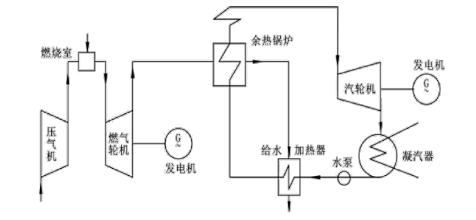
\includegraphics[width=0.82\textwidth]{chapter1/燃气蒸汽联合循环示意图.png}
  \caption{Schematic diagram of the gas--steam combined cycle system.}
  \label{fig:ccpp-schematic}
\end{figure}

\section{Data-Driven Thermodynamic Modeling Methods}

\subsection{Unified Working-Fluid Stream Model}

Different working fluids coexist in the combined cycle, including fuel gas, humid air, combustion products, water and steam. To provide a common data interface for component models, each flow path is represented as a stream object:
\begin{equation}
\mathcal{F}_k
=
\left\{
\dot{m}_k,\,
T_k,\,
P_k,\,
h_k,\,
s_k,\,
\boldsymbol{x}_k,\,
e_{x,k}
\right\},
\label{eq:stream}
\end{equation}
where \(\dot{m}\), \(T\), \(P\), \(h\), \(s\), \(\boldsymbol{x}\) and \(e_x\) denote mass flow rate, temperature, pressure, specific enthalpy, specific entropy, composition and specific exergy, respectively. The specific exergy relative to the reference environment is
\begin{equation}
e_{x,k} = (h_k-h_{0,k}) - T_0(s_k-s_{0,k}).
\label{eq:exergy}
\end{equation}

For a steady-flow component with negligible kinetic and potential energy changes, the energy balance is written as
\begin{equation}
\dot{Q}-\dot{W}
+\sum_{\mathrm{in}}\dot{m}_{\mathrm{in}}h_{\mathrm{in}}
-\sum_{\mathrm{out}}\dot{m}_{\mathrm{out}}h_{\mathrm{out}}=0.
\label{eq:energy-balance}
\end{equation}
The corresponding exergy balance is
\begin{equation}
\sum_{\mathrm{in}}\dot{E}_{x,\mathrm{in}}
-\sum_{\mathrm{out}}\dot{E}_{x,\mathrm{out}}
+\sum_j\left(1-\frac{T_0}{T_j}\right)\dot{Q}_j
-\dot{W}
=\dot{E}_{x,\mathrm{dest}}.
\label{eq:exergy-balance}
\end{equation}

Gas-mixture properties are calculated from component composition with normalization of fuel composition, humidity correction for inlet air and stoichiometric combustion calculation for flue gas. Water and steam properties are obtained from IAPWS-IF97 using \((P,T)\), \((P,x)\), \((P,h)\) or \((P,s)\) input pairs. In the field-data implementation, one operating row can construct up to 66 stream objects: 56 water/steam streams and 10 gas-side streams. The modeling logic is summarized in Fig.~\ref{fig:fluid-model}.

\begin{figure}[H]
  \centering
  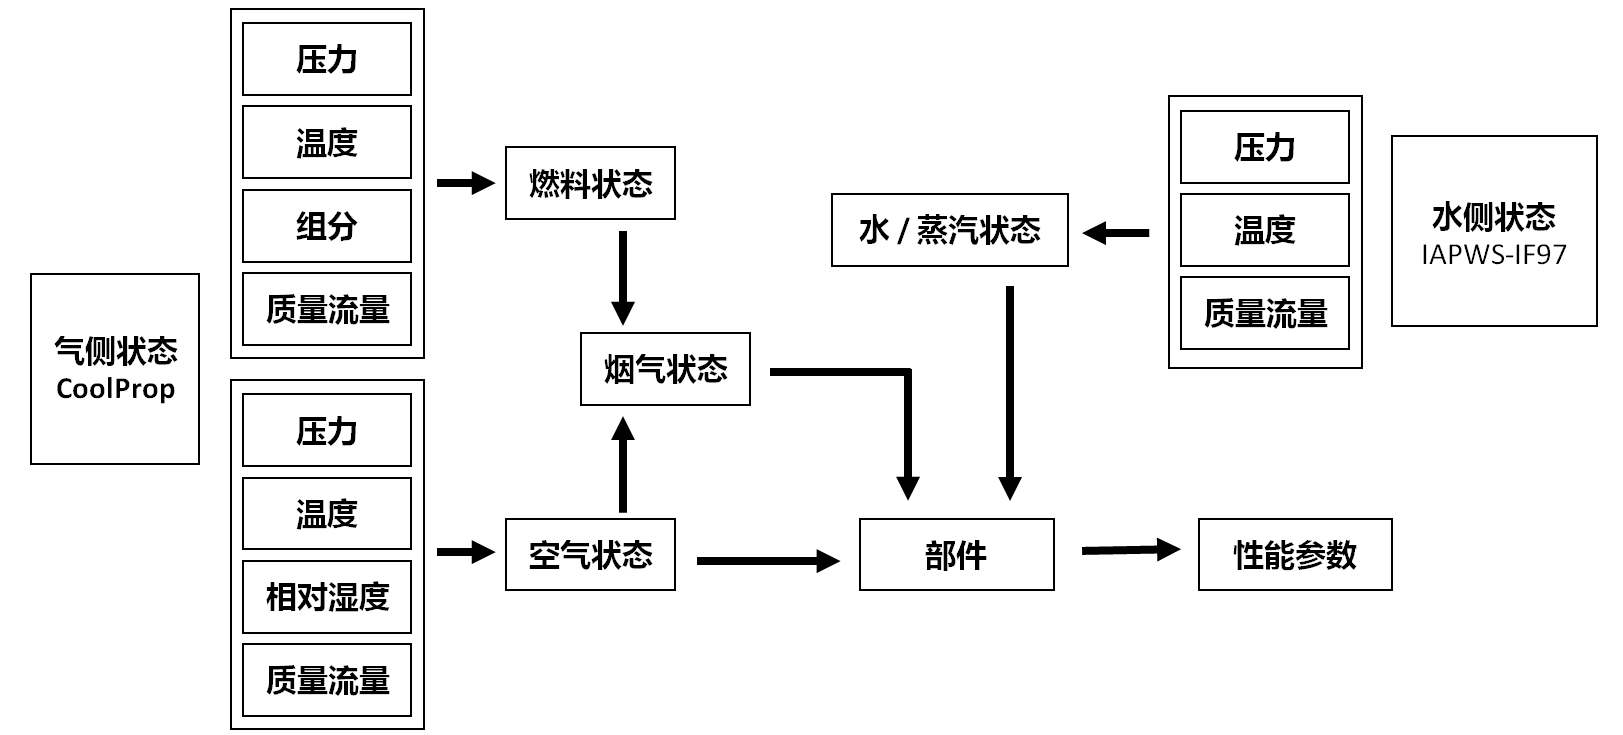
\includegraphics[width=0.82\textwidth]{chapter2/工质建模示意图.png}
  \caption{Unified stream-based working-fluid modeling framework.}
  \label{fig:fluid-model}
\end{figure}

\subsection{Gas Turbine Model}

The gas turbine is divided into compressor, combustor and turbine control volumes. For the compressor, the isentropic outlet state \(2s\) satisfies
\begin{equation}
P_{2s}=P_2,\qquad s_{2s}=s_1.
\end{equation}
Considering a parameterized cooling bleed fraction \(\beta_b\), the bleed and main-flow mass rates are
\begin{equation}
\dot{m}_b=\beta_b\dot{m}_1,\qquad
\dot{m}_{2,\mathrm{main}}=(1-\beta_b)\dot{m}_1.
\end{equation}
The compressor isentropic efficiency and power consumption are
\begin{equation}
\eta_{c,s}=\frac{h_{2s}-h_1}{h_2-h_1},
\qquad
\dot{W}_c=\dot{m}_{2,\mathrm{main}}h_2+\dot{m}_b h_b-\dot{m}_1h_1.
\label{eq:compressor}
\end{equation}

In the combustor, the fuel lower heating value is obtained by composition weighting. With combustion efficiency \(\eta_{\mathrm{comb}}\), the released heat is
\begin{equation}
\dot{Q}_{\mathrm{rel}}=\eta_{\mathrm{comb}} LHV_f \dot{m}_f.
\end{equation}
The combustor outlet enthalpy is calculated from
\begin{equation}
h_3=
\frac{\dot{m}_{2,\mathrm{main}}h_2+\dot{m}_f h_f+\dot{Q}_{\mathrm{rel}}}
{\dot{m}_{2,\mathrm{main}}+\dot{m}_f}.
\label{eq:combustor}
\end{equation}

Cooling-air mixing before turbine expansion is treated as an equivalent adiabatic mixing process:
\begin{equation}
h_{3c}=
\frac{\dot{m}_3 h_3+\dot{m}_b h_b}{\dot{m}_3+\dot{m}_b}.
\end{equation}
The turbine isentropic outlet state \(4s\) satisfies \(P_{4s}=P_4\) and \(s_{4s}=s_{3c}\). The turbine isentropic efficiency and output power are
\begin{equation}
\eta_{t,s}=\frac{h_{3c}-h_4}{h_{3c}-h_{4s}},
\qquad
\dot{W}_t=\dot{m}_{3c}(h_{3c}-h_4).
\label{eq:turbine}
\end{equation}

\subsection{HRSG and Steam Turbine Models}

Because detailed heat-transfer-surface measurements are limited, each HRSG is modeled from whole-unit gas-side heat release and water-side heat absorption. For HRSG \(j\),
\begin{equation}
\dot{Q}_{g,j}
=\dot{m}_{g,\mathrm{in}}h_{g,\mathrm{in}}
-\dot{m}_{g,\mathrm{out}}h_{g,\mathrm{out}},
\end{equation}
\begin{equation}
\dot{Q}_{w,j}
=
\sum_{o\in\mathcal{W}_{j,\mathrm{out}}}\dot{m}_oh_o
-
\sum_{i\in\mathcal{W}_{j,\mathrm{in}}}\dot{m}_ih_i.
\end{equation}
The HRSG heat-transfer efficiency and exhaust-gas energy-release effectiveness are
\begin{equation}
\eta_{\mathrm{HRSG},j}=\frac{\dot{Q}_{w,j}}{\dot{Q}_{g,j}},
\qquad
\varepsilon_{\mathrm{HRSG},j}
=\frac{\dot{Q}_{g,j}}{\dot{m}_{g,\mathrm{in}}h_{g,\mathrm{in}}}.
\label{eq:hrsg}
\end{equation}

The steam turbine is divided into high-pressure (HP), intermediate-pressure (IP) and low-pressure (LP) cylinders. For cylinder \(k\), the isentropic outlet state satisfies
\begin{equation}
P_{k,s}=P_{k,\mathrm{out}},\qquad s_{k,s}=s_{k,\mathrm{in}}.
\end{equation}
Cylinder output and isentropic efficiency are
\begin{equation}
\dot{W}_k=\dot{m}_{k,\mathrm{in}}(h_{k,\mathrm{in}}-h_{k,\mathrm{out}}),
\qquad
\eta_{k,s}=
\frac{h_{k,\mathrm{in}}-h_{k,\mathrm{out}}}
{h_{k,\mathrm{in}}-h_{k,s}}.
\label{eq:st-cylinder}
\end{equation}
The calculated steam turbine output is
\begin{equation}
\dot{W}_{\mathrm{ST,cal}}
=\dot{W}_{\mathrm{HP}}+\dot{W}_{\mathrm{IP}}+\dot{W}_{\mathrm{LP}}.
\label{eq:st-total}
\end{equation}
During heating operation, part of the low-pressure steam is supplied to the heat network, which reduces LP turbine flow and changes the relationship between electric output and total useful output.

\subsection{Correlation Analysis}

Pearson correlation analysis is used to screen variables associated with plant efficiency. Non-heating operation uses combined-cycle power-generation efficiency as the dependent variable, while heating operation uses heat-electricity efficiency:
\begin{equation}
\eta_{\mathrm{he}}=\frac{W_e+Q_h}{Q_f}.
\label{eq:heat-electricity}
\end{equation}
The correlation coefficient is only a measure of linear association. It does not prove causality and can be affected by load scheduling, seasonality and multicollinearity. Therefore, correlation results are interpreted together with thermodynamic mechanisms and scatter-plot trends.

\section{Results and Discussion}

\subsection{Gas Turbine Performance}

The calculated output of both gas turbines generally follows the measured output, indicating that the stream-based gas turbine model can reproduce the main energy conversion process. Remaining deviations are larger in winter operating points, mainly because the air-flow correction parameters are fitted primarily from summer conditions and the gas turbine becomes more sensitive to air-flow uncertainty at low ambient temperature.

\begin{figure}[H]
  \centering
  \begin{subfigure}{0.48\textwidth}
    \centering
    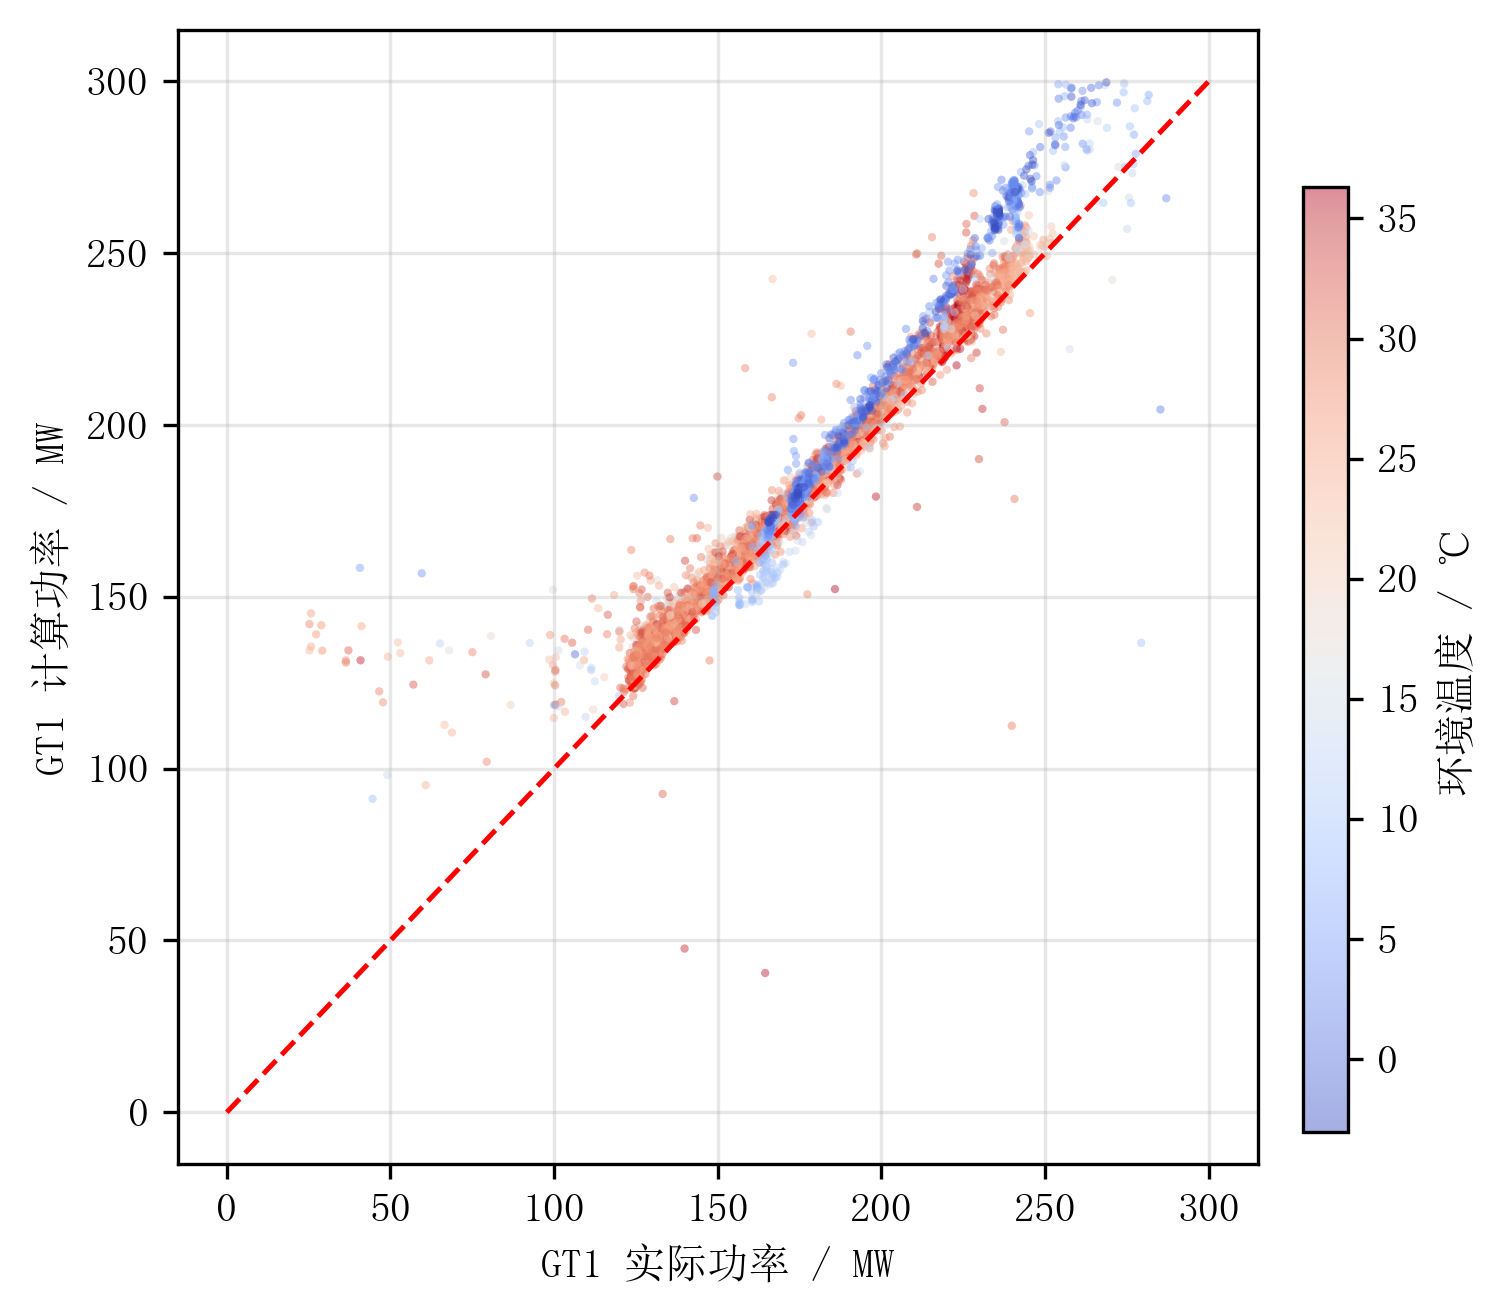
\includegraphics[width=\textwidth]{chapter3/1燃机1出力.png}
    \caption{\#1 gas turbine.}
  \end{subfigure}
  \hfill
  \begin{subfigure}{0.48\textwidth}
    \centering
    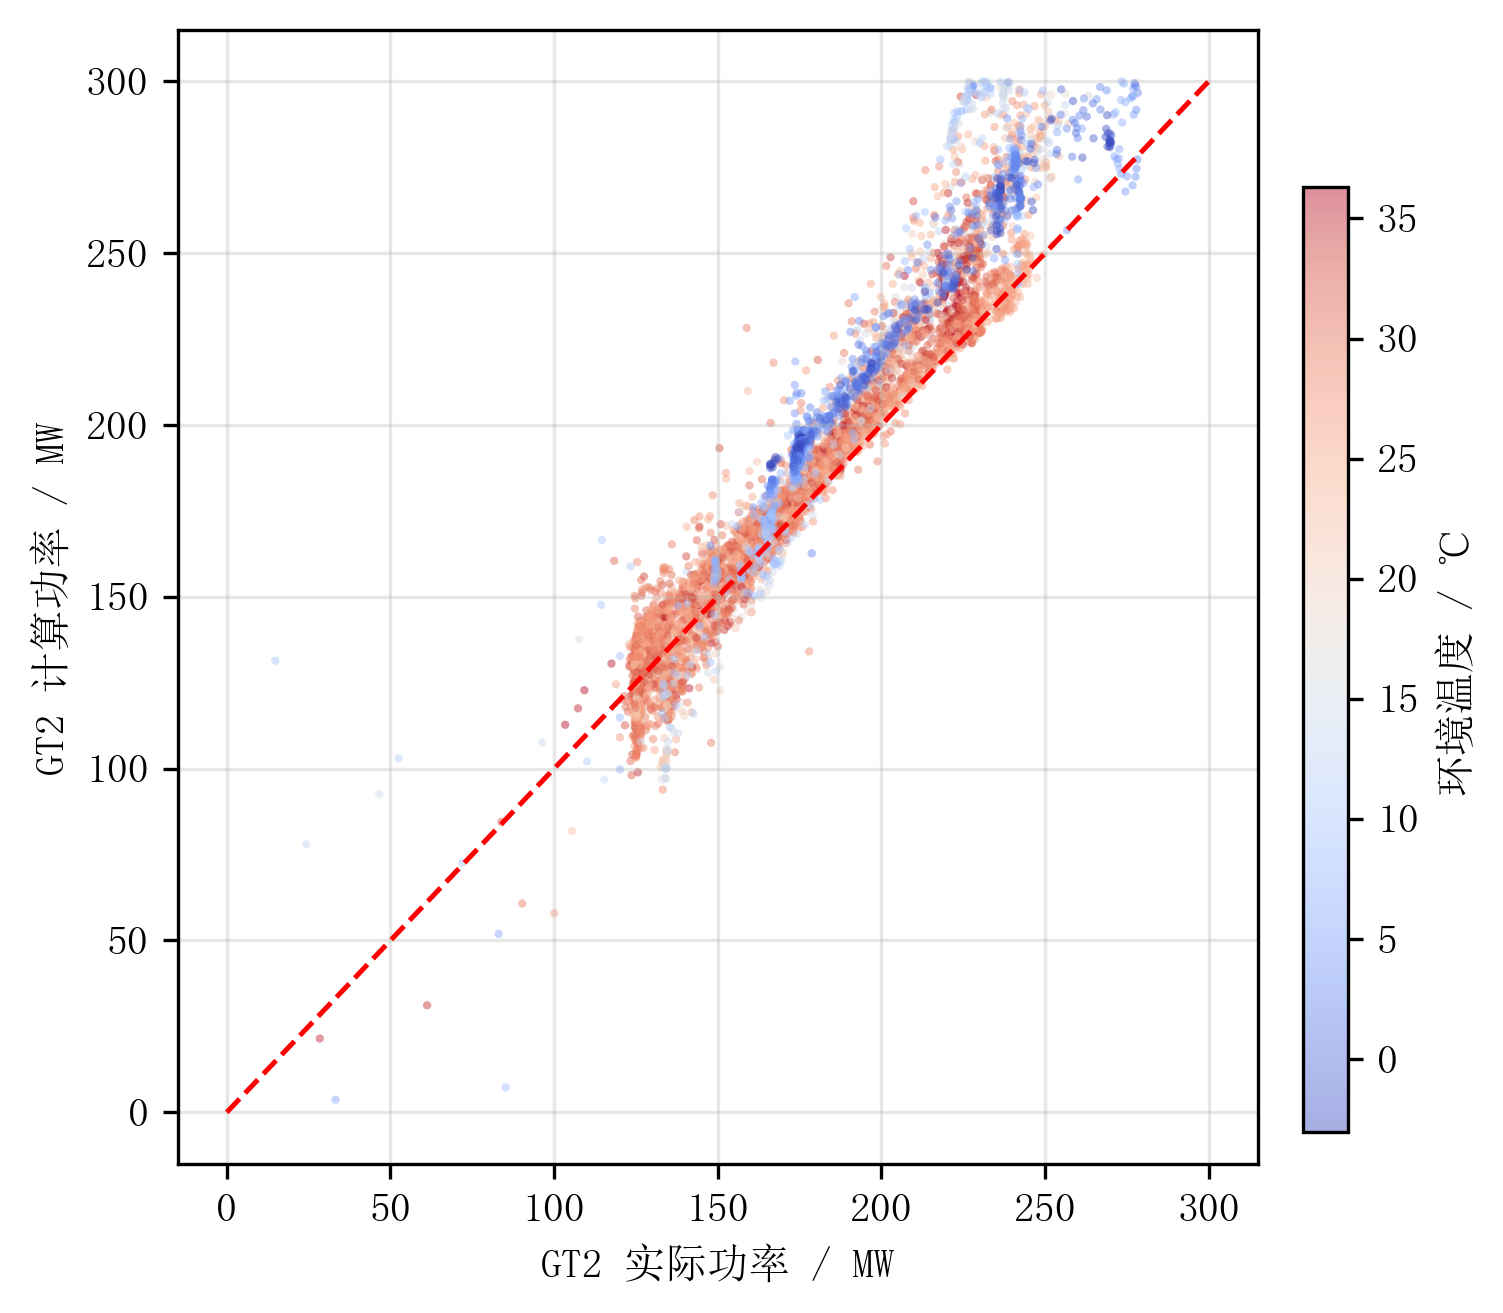
\includegraphics[width=\textwidth]{chapter3/1燃机2出力.png}
    \caption{\#2 gas turbine.}
  \end{subfigure}
  \caption{Comparison between calculated and measured gas turbine output.}
  \label{fig:gt-output}
\end{figure}

The gas turbine energy-share results show that approximately \(0.28\)--\(0.36\) of the fuel input is converted into electric output, and this share increases slightly with gas turbine load. Compressor power consumption accounts for about \(0.38\)--\(0.43\) of fuel input. Exhaust heat and other losses account for about \(0.22\)--\(0.32\), indicating significant bottoming-cycle heat-recovery potential. Therefore, gas turbine exhaust energy should not be interpreted as a simple loss in the combined-cycle context; it is the heat source that determines HRSG steam generation and steam turbine output.

\begin{figure}[H]
  \centering
  \begin{subfigure}{0.48\textwidth}
    \centering
    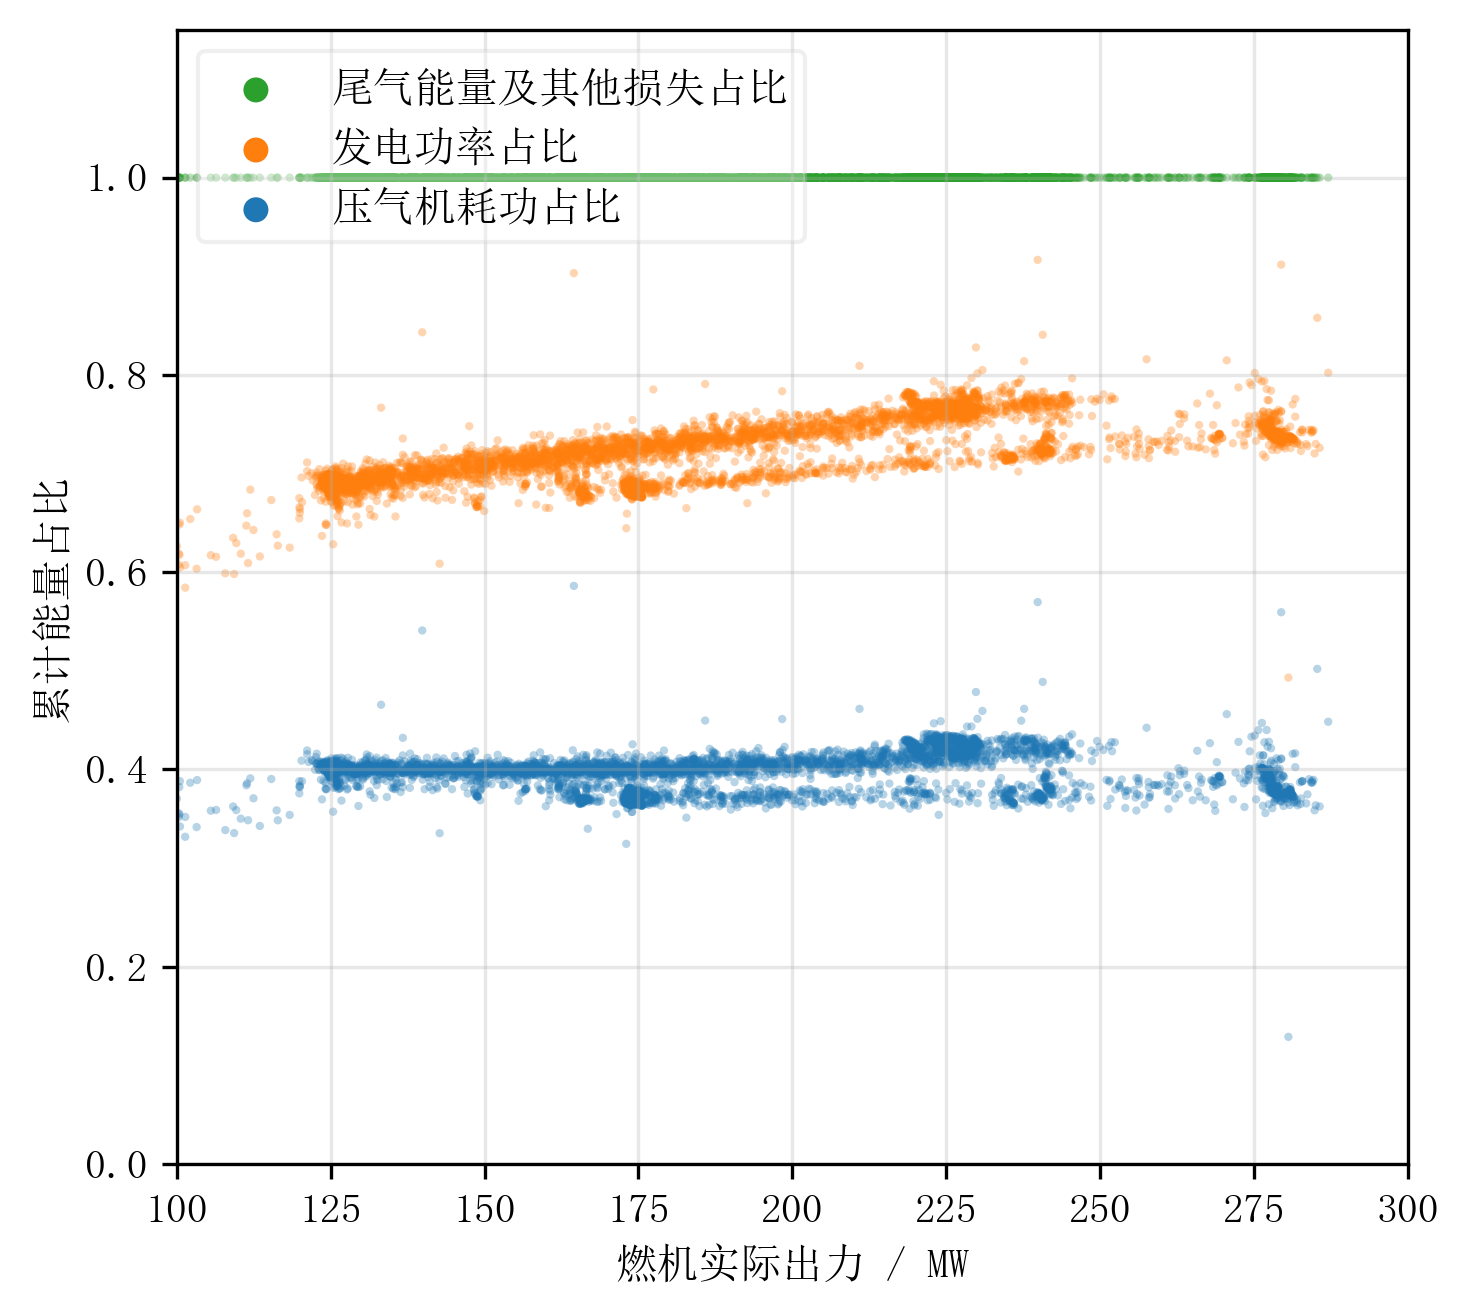
\includegraphics[width=\textwidth]{chapter3/2-1GT1能量占比.png}
    \caption{\#1 gas turbine.}
  \end{subfigure}
  \hfill
  \begin{subfigure}{0.48\textwidth}
    \centering
    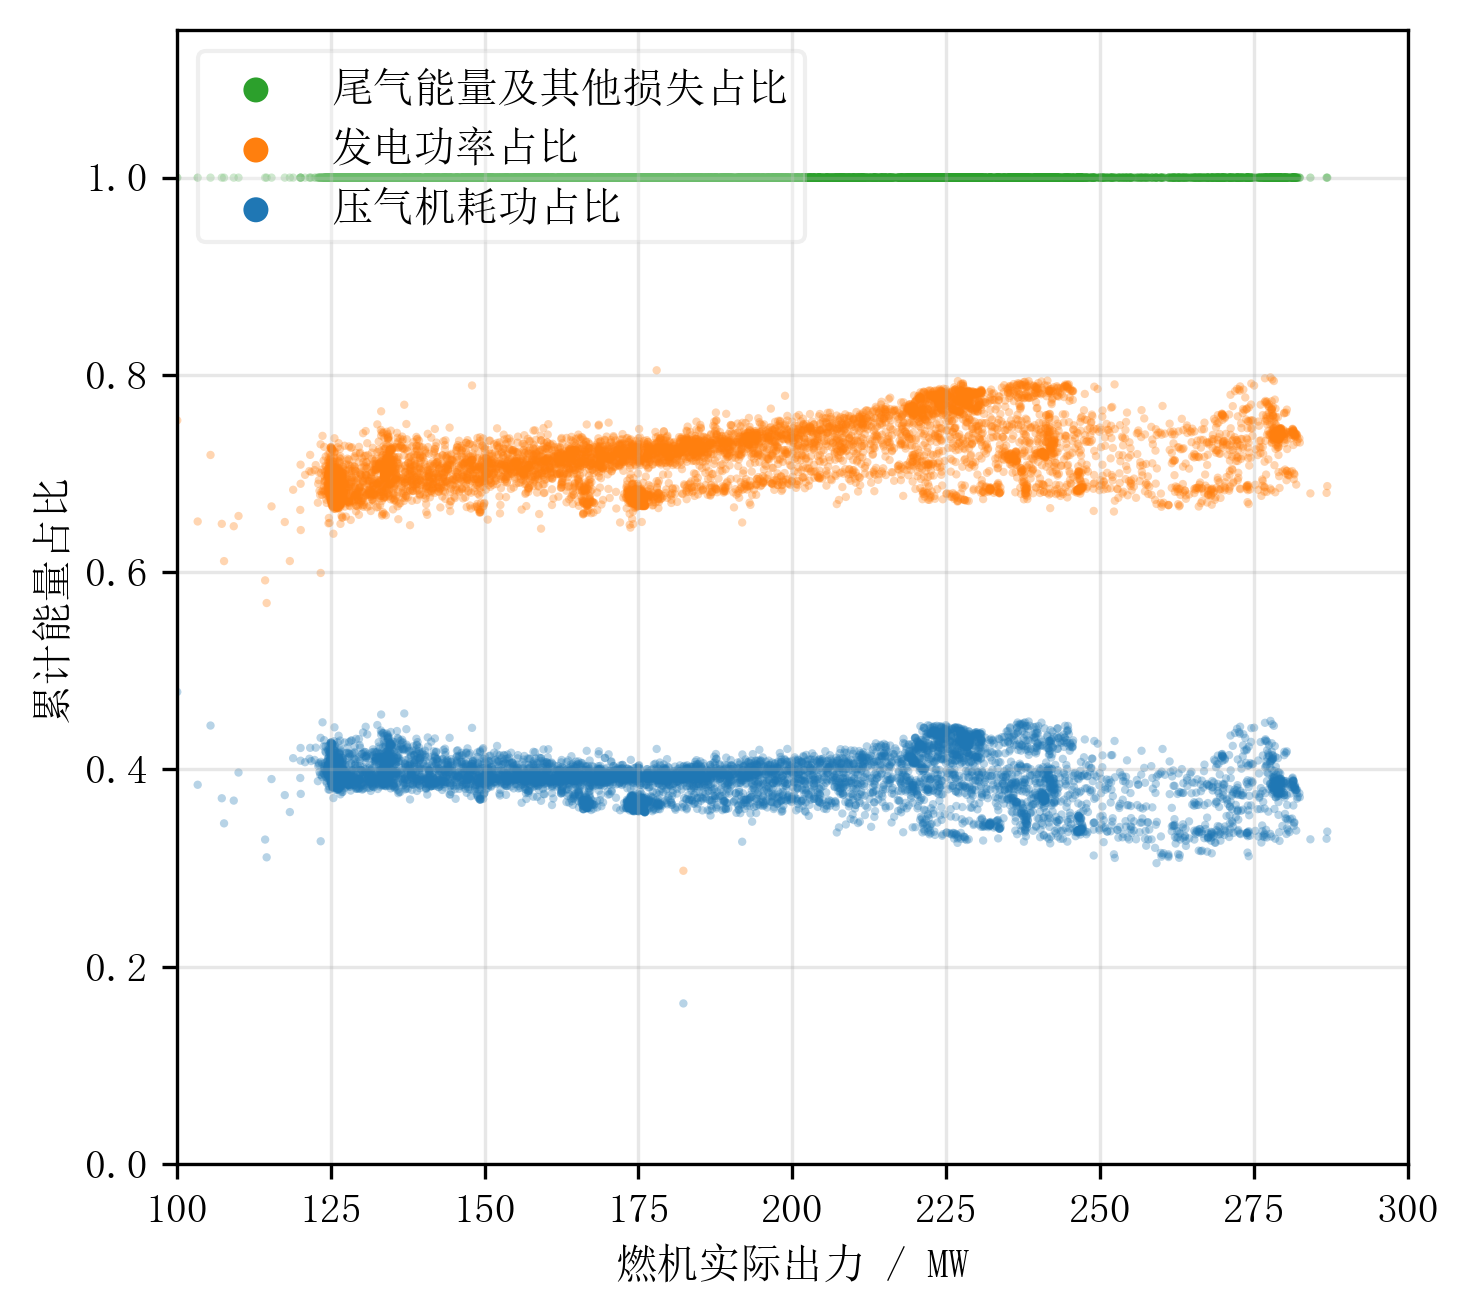
\includegraphics[width=\textwidth]{chapter3/2-1GT2能量占比.png}
    \caption{\#2 gas turbine.}
  \end{subfigure}
  \caption{Gas turbine energy-share distribution.}
  \label{fig:gt-energy-share}
\end{figure}

\subsection{HRSG Heat Recovery and Steam Turbine Output}

The HRSG gas-side energy distribution shows several typical operating regions. Low output around \(75\)--\(100\) MW mainly corresponds to one-on-one operation without heating. Medium output around \(100\)--\(125\) MW is often associated with two-on-one heating operation, in which both gas turbines operate but low-pressure steam is redirected to the heat network. High output corresponds to two-on-one non-heating or low-heating operation with high gas turbine exhaust energy and high steam turbine output.

\begin{figure}[H]
  \centering
  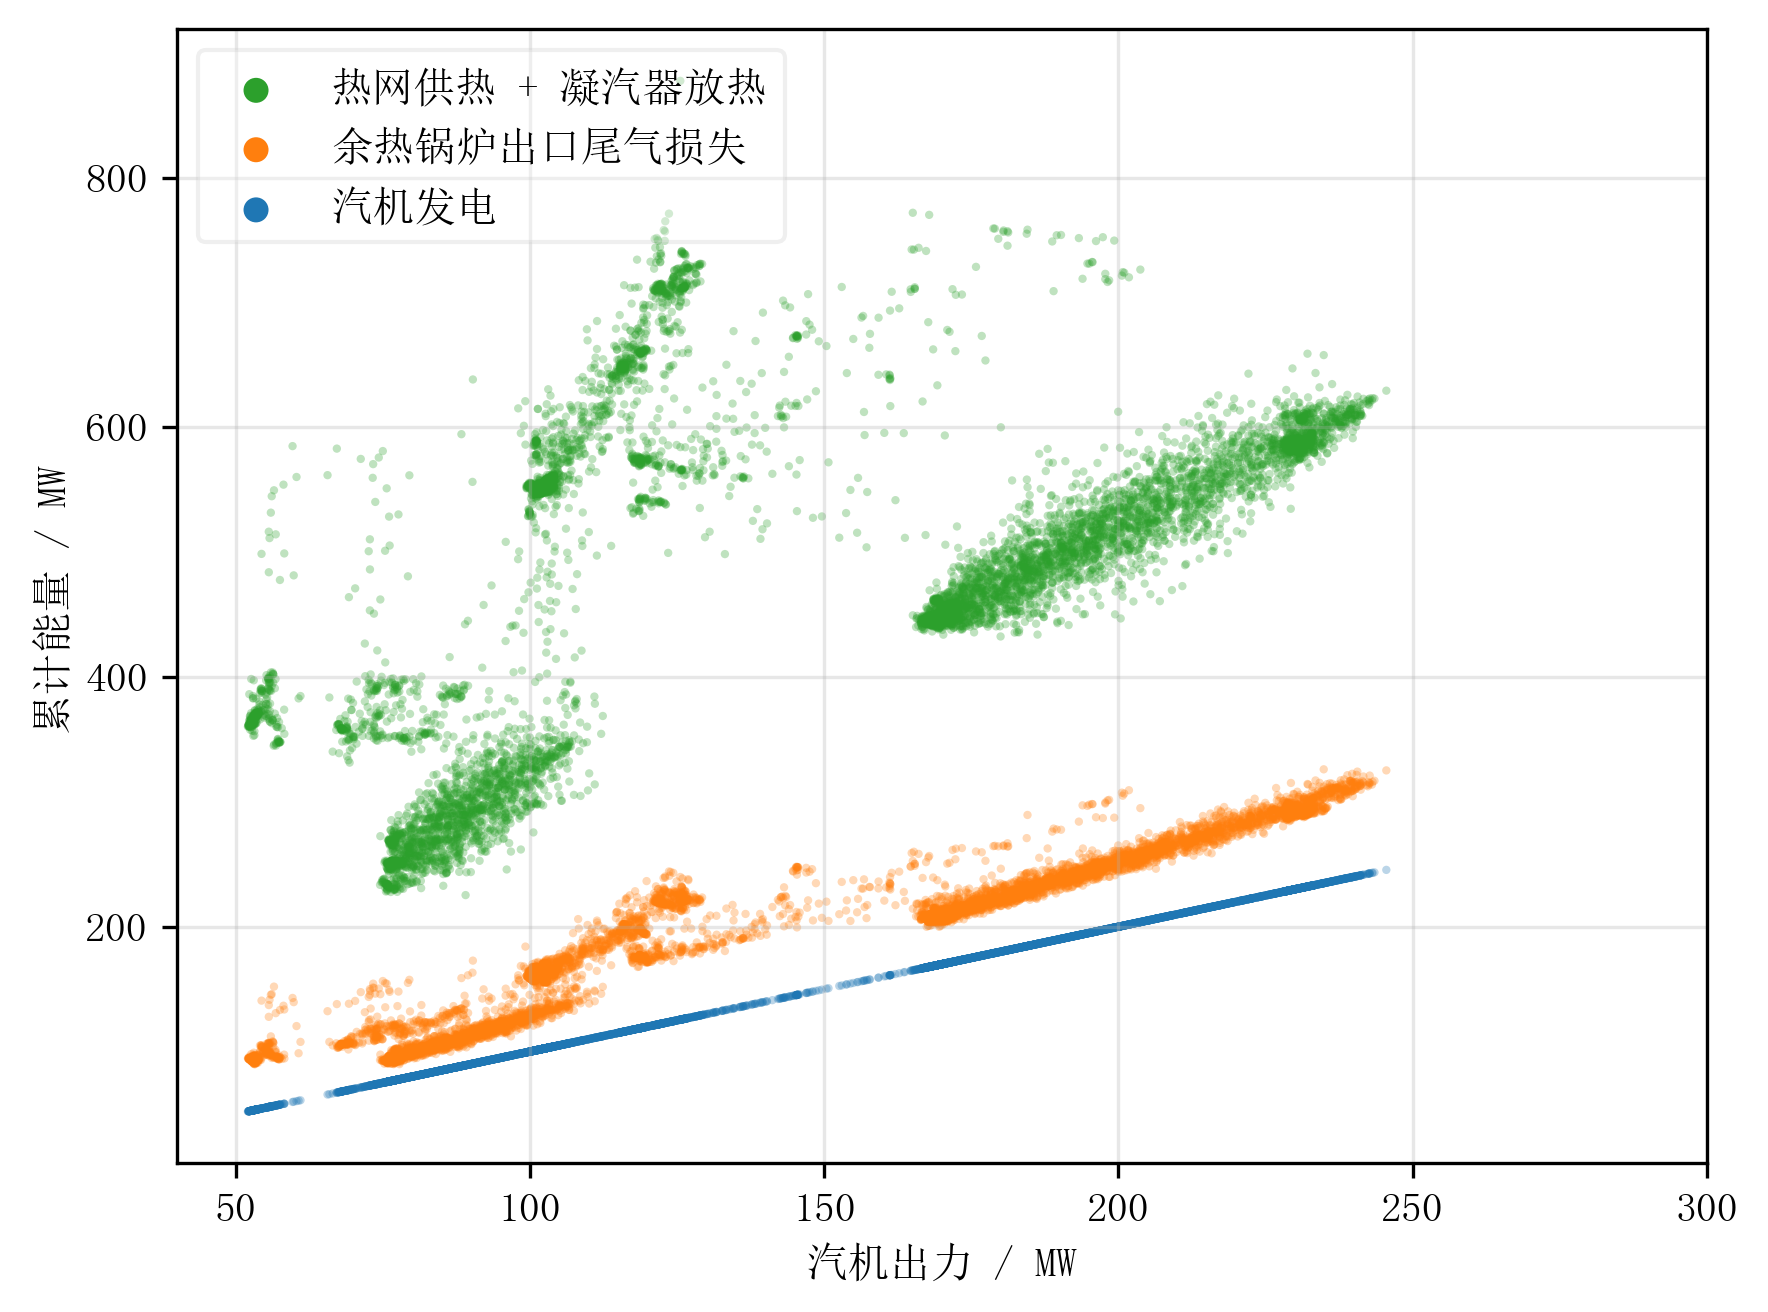
\includegraphics[width=0.78\textwidth]{chapter4/1烟气能量分配.png}
  \caption{Gas-side energy distribution of the HRSGs.}
  \label{fig:hrsg-gas-energy}
\end{figure}

On the water/steam side, heat absorption at different pressure levels increases almost linearly with plant output. The high-pressure steam system contributes the largest share, approximately \(0.56\)--\(0.64\), making it the dominant part of HRSG water-side heat absorption. The intermediate-pressure and reheating systems account for about \(0.22\)--\(0.30\), while low-pressure steam accounts for about \(0.12\)--\(0.18\) and becomes more important at high load. These trends indicate that high-pressure steam generation is central to bottoming-cycle power generation, while low-pressure steam has a strong effect on heating operation and high-load heat recovery.

\begin{figure}[H]
  \centering
  \begin{subfigure}{0.48\textwidth}
    \centering
    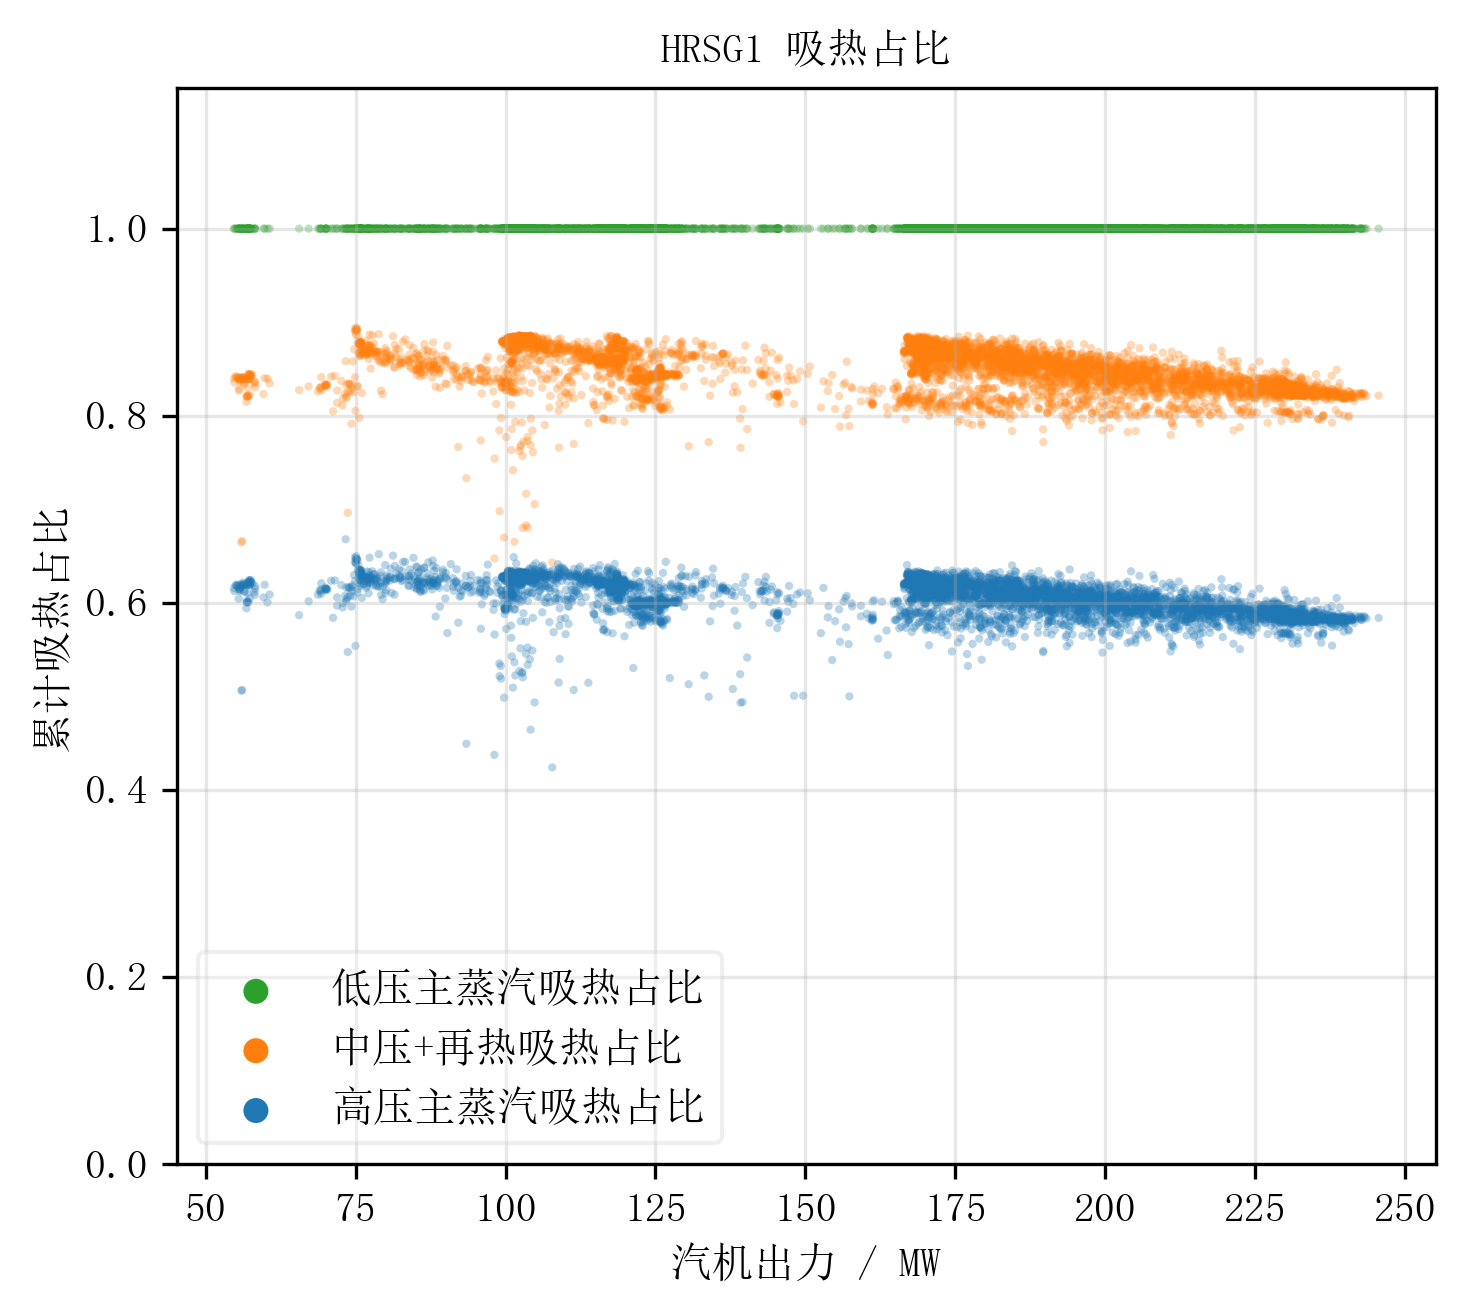
\includegraphics[width=\textwidth]{chapter4/2-1HRSG1吸热占比.png}
    \caption{\#1 HRSG.}
  \end{subfigure}
  \hfill
  \begin{subfigure}{0.48\textwidth}
    \centering
    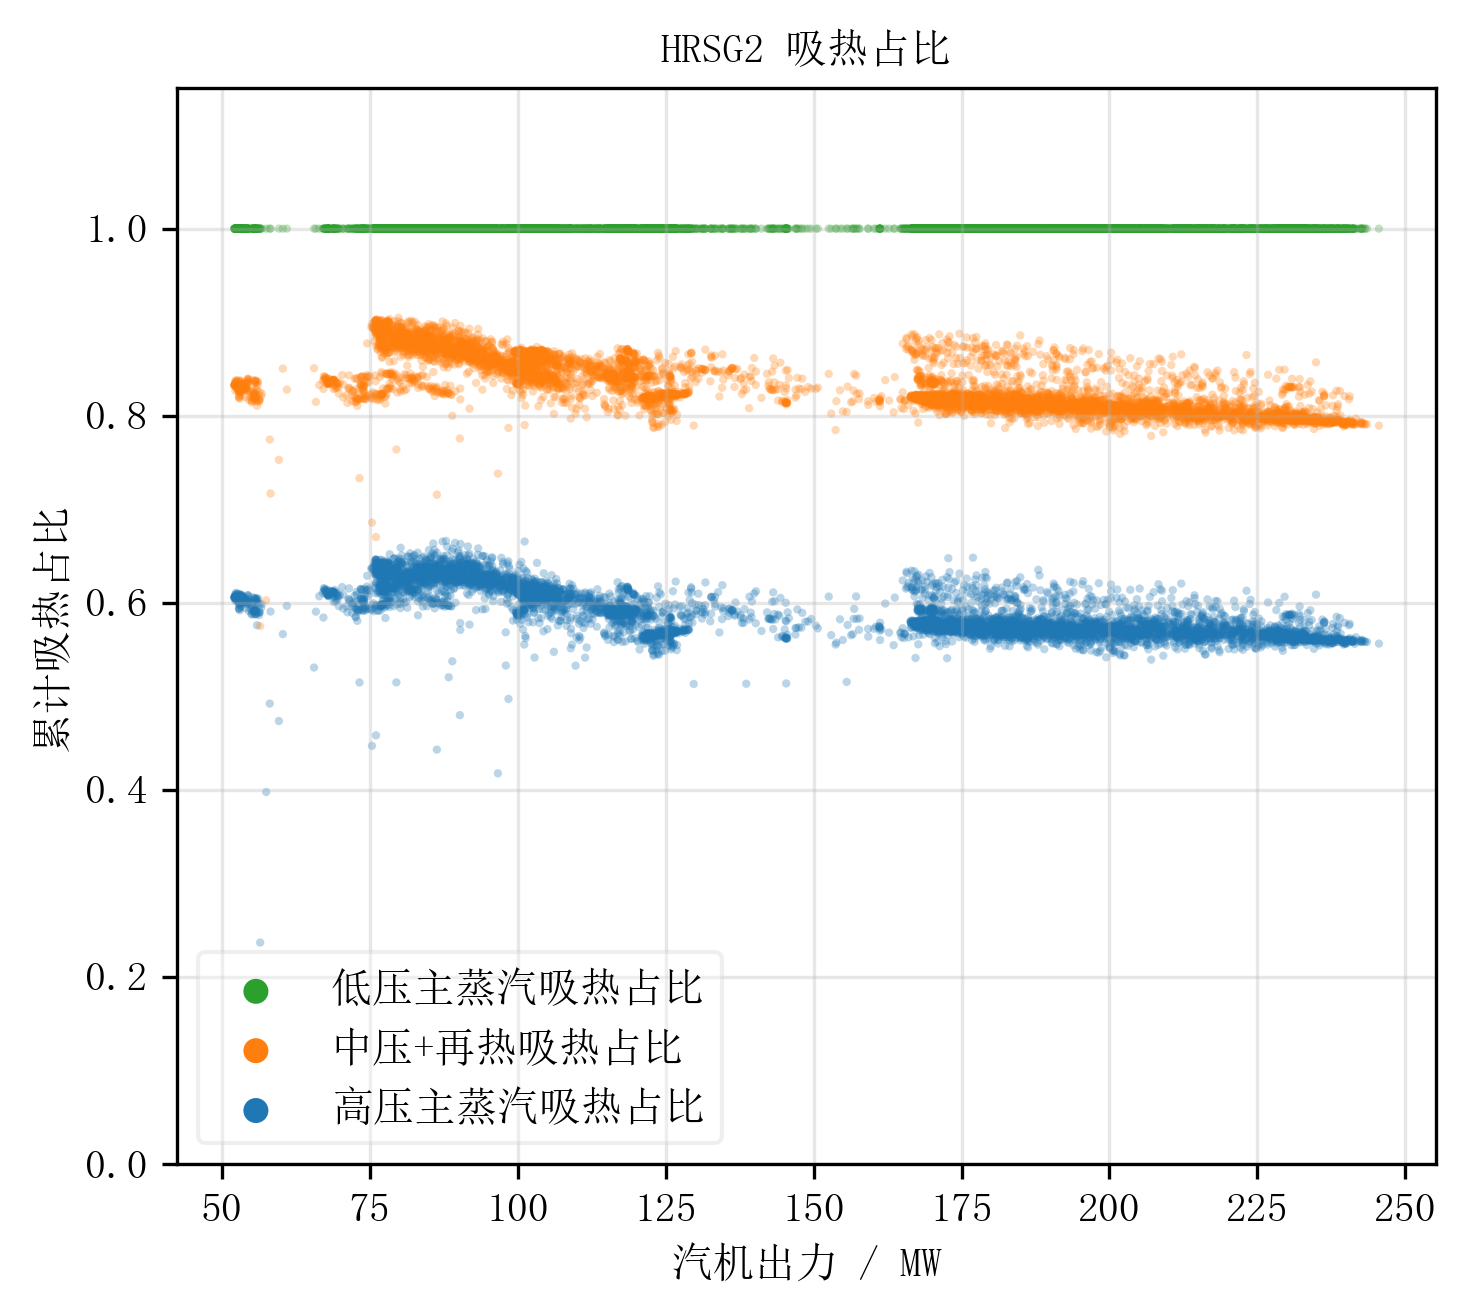
\includegraphics[width=\textwidth]{chapter4/2-1HRSG2吸热占比.png}
    \caption{\#2 HRSG.}
  \end{subfigure}
  \caption{Water-side heat absorption share of the HRSGs.}
  \label{fig:hrsg-water-share}
\end{figure}

The steam turbine model reproduces measured power trends. The calculated power is slightly higher before correction, mainly because shaft-seal extraction, mechanical efficiency and small heating extraction flows are difficult to quantify from the available measurements. The cylinder power distribution further shows that LP cylinder contribution is high in non-heating high-load operation but decreases significantly during heating operation because steam is transferred to the heat network.

\begin{figure}[H]
  \centering
  \begin{subfigure}{0.48\textwidth}
    \centering
    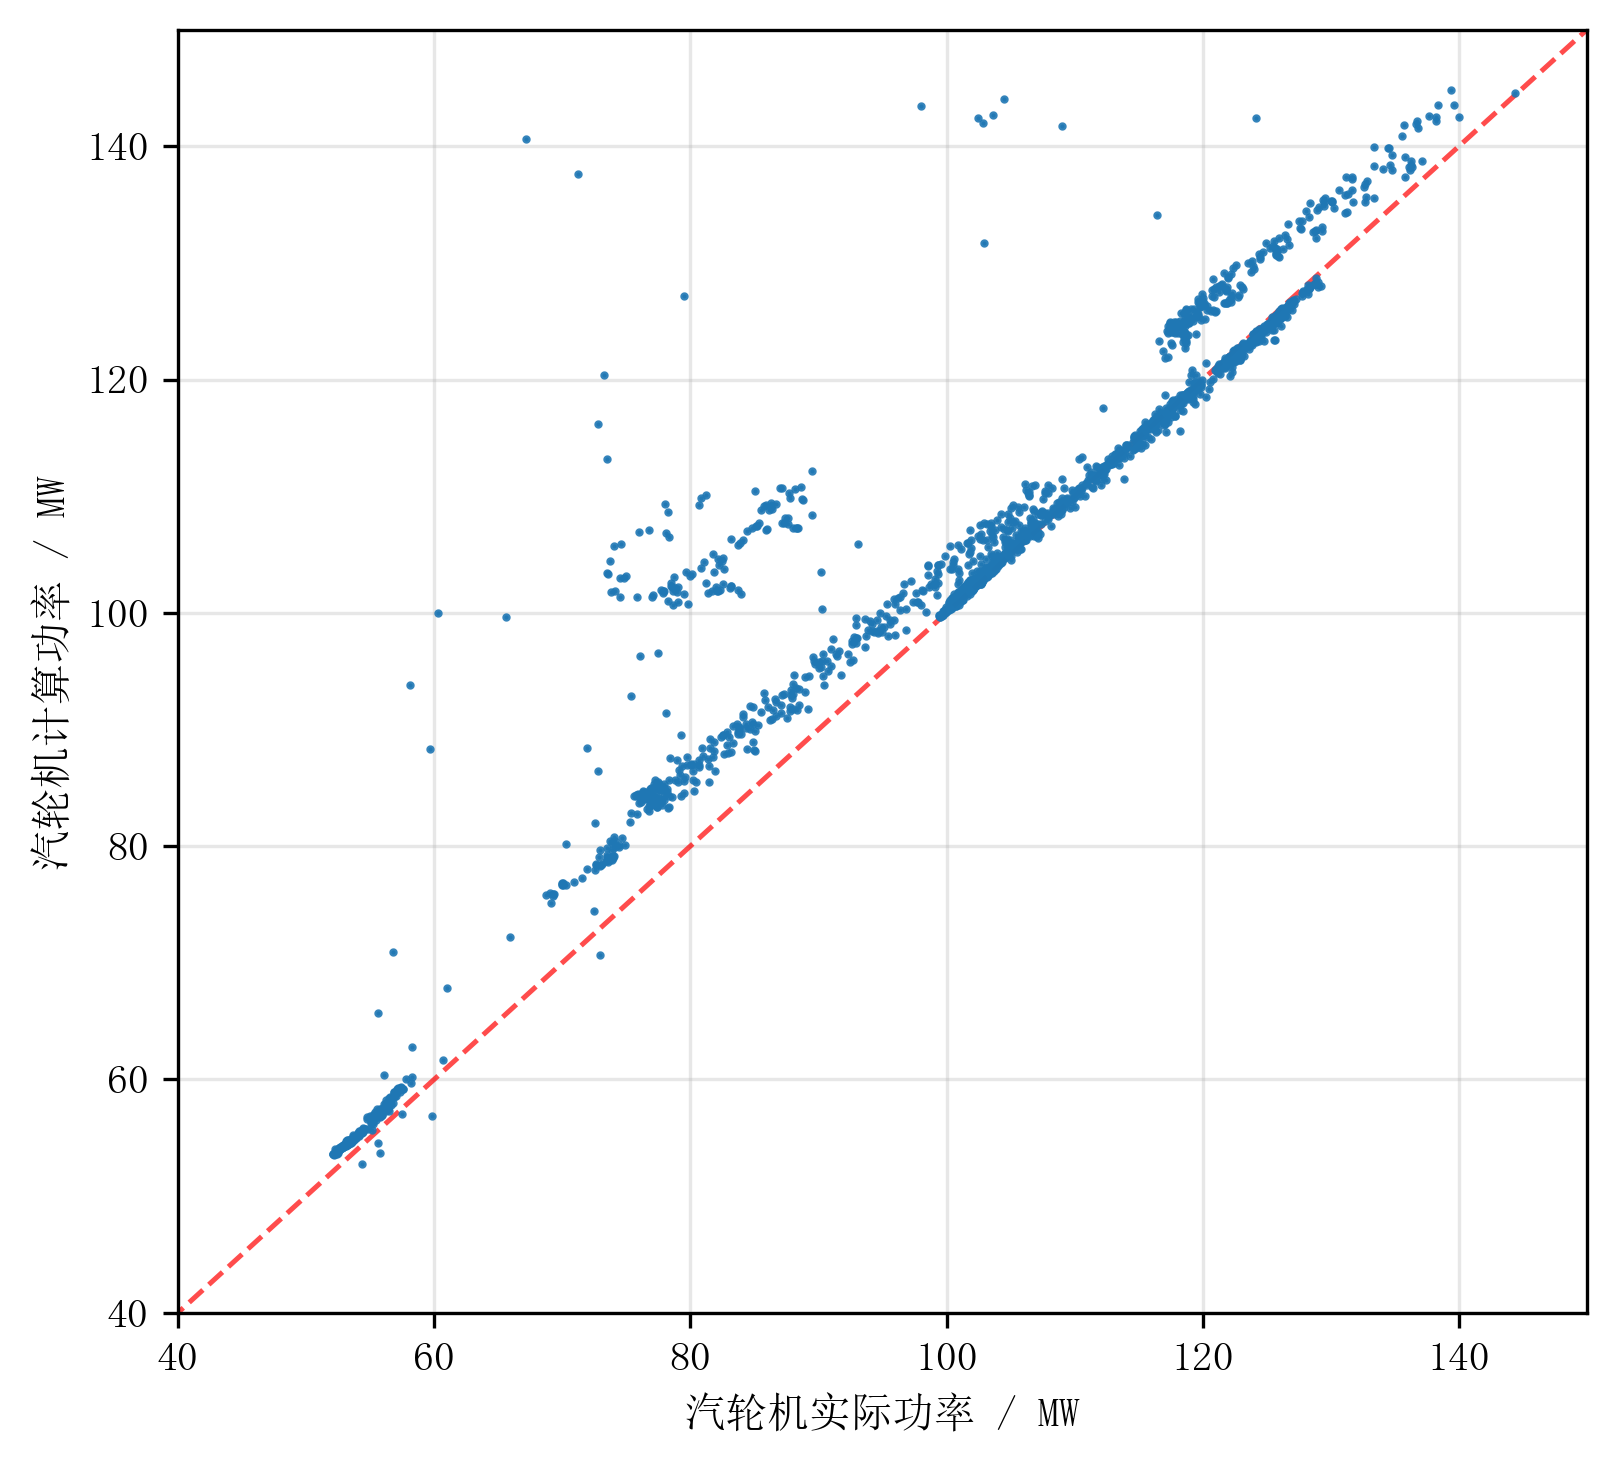
\includegraphics[width=\textwidth]{chapter4/3汽机出力计算.png}
    \caption{Steam turbine output.}
  \end{subfigure}
  \hfill
  \begin{subfigure}{0.48\textwidth}
    \centering
    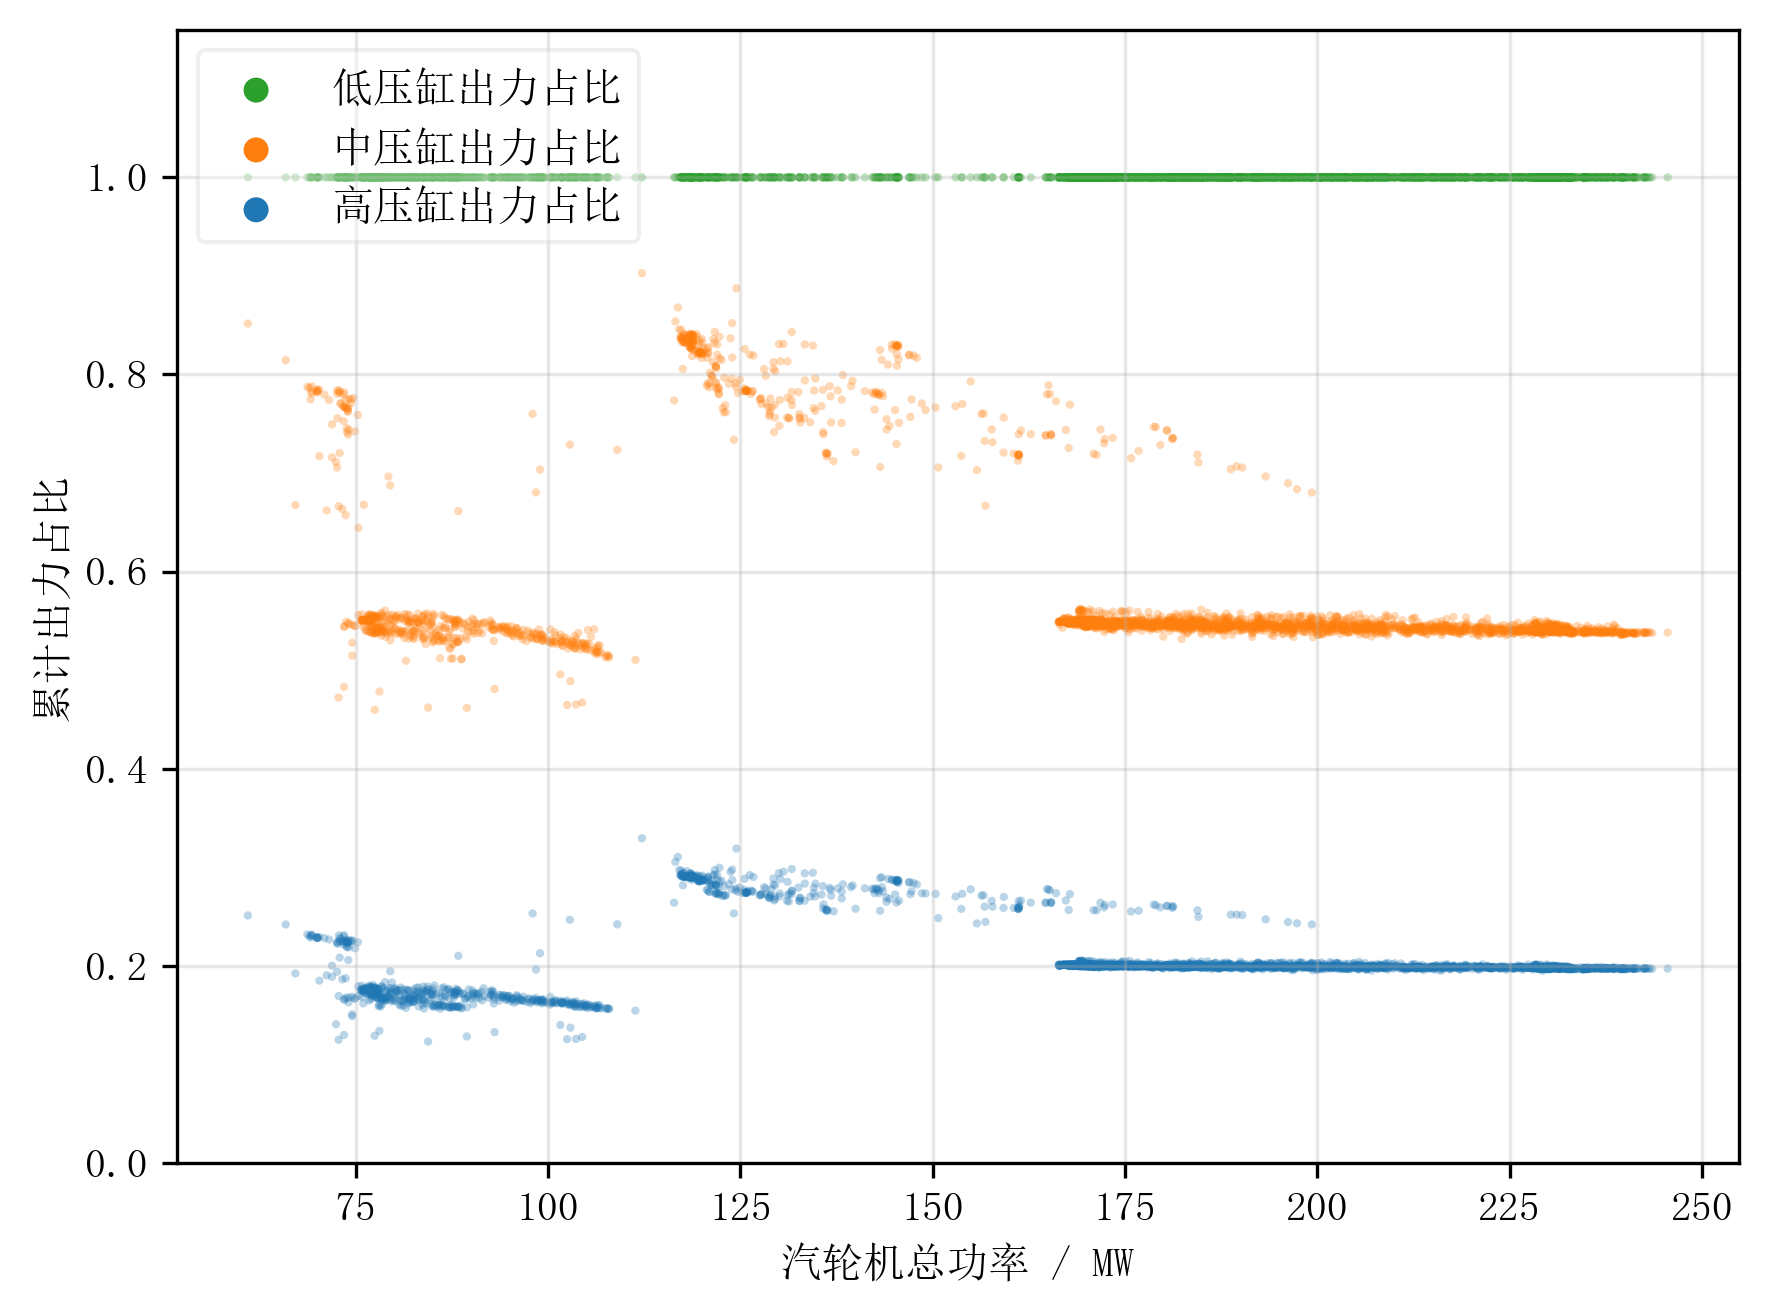
\includegraphics[width=\textwidth]{chapter4/4-1各缸出力占比.png}
    \caption{Cylinder output share.}
  \end{subfigure}
  \caption{Steam turbine power calculation and cylinder power distribution.}
  \label{fig:st-output}
\end{figure}

\subsection{Efficiency-Related Variables}

Table~\ref{tab:corr} lists the ten variables with the largest absolute Pearson correlation coefficients under non-heating and heating conditions. The results confirm that the two operating modes have different efficiency mechanisms. In non-heating operation, efficiency is mainly related to steam turbine output, total load, main-steam flow and feedwater pressure, which represent the ability of the bottoming cycle to convert recovered exhaust heat into electric power. In heating operation, heat supply dominates because the efficiency definition includes useful heat output.

\begin{table}[H]
  \centering
  \caption{Main variables associated with combined-cycle efficiency under different operating modes.}
  \label{tab:corr}
  \small
  \begin{tabular}{lrlr}
    \toprule
    \multicolumn{2}{c}{Non-heating power efficiency} &
    \multicolumn{2}{c}{Heating heat-electricity efficiency} \\
    Variable & \(r\) & Variable & \(r\) \\
    \midrule
    Steam turbine output & 0.621 & Heating load & 0.966 \\
    Ambient pressure & -0.528 & Ambient temperature & -0.930 \\
    Ambient temperature & 0.481 & Ambient pressure & 0.781 \\
    Low-pressure feedwater pressure & 0.474 & Steam turbine output & -0.739 \\
    Combined-cycle electric power & 0.466 & Ambient humidity & -0.710 \\
    High-pressure main steam flow & 0.428 & Air flow rate & 0.386 \\
    High-pressure feedwater pressure & 0.412 & Total gas turbine output & 0.355 \\
    Intermediate-pressure main steam flow & 0.410 & Low-pressure feedwater pressure & -0.348 \\
    Intermediate-pressure feedwater pressure & 0.405 & High-pressure feedwater pressure & 0.200 \\
    Turbine exhaust temperature & 0.398 & Intermediate-pressure main steam flow & 0.192 \\
    \bottomrule
  \end{tabular}
\end{table}

The scatter relationships in Fig.~\ref{fig:load-efficiency} show that gas turbine output, steam turbine output and total plant electric power are positively associated with power-generation efficiency in non-heating operation. This is because high-load operation increases exhaust gas temperature and flow rate, improves steam generation and moves the steam turbine closer to its design flow condition. In contrast, heating load is almost linearly associated with heat-electricity efficiency under heating operation because heat output is directly included in the numerator of Eq.~\eqref{eq:heat-electricity}.

\begin{figure}[H]
  \centering
  \begin{subfigure}{0.48\textwidth}
    \centering
    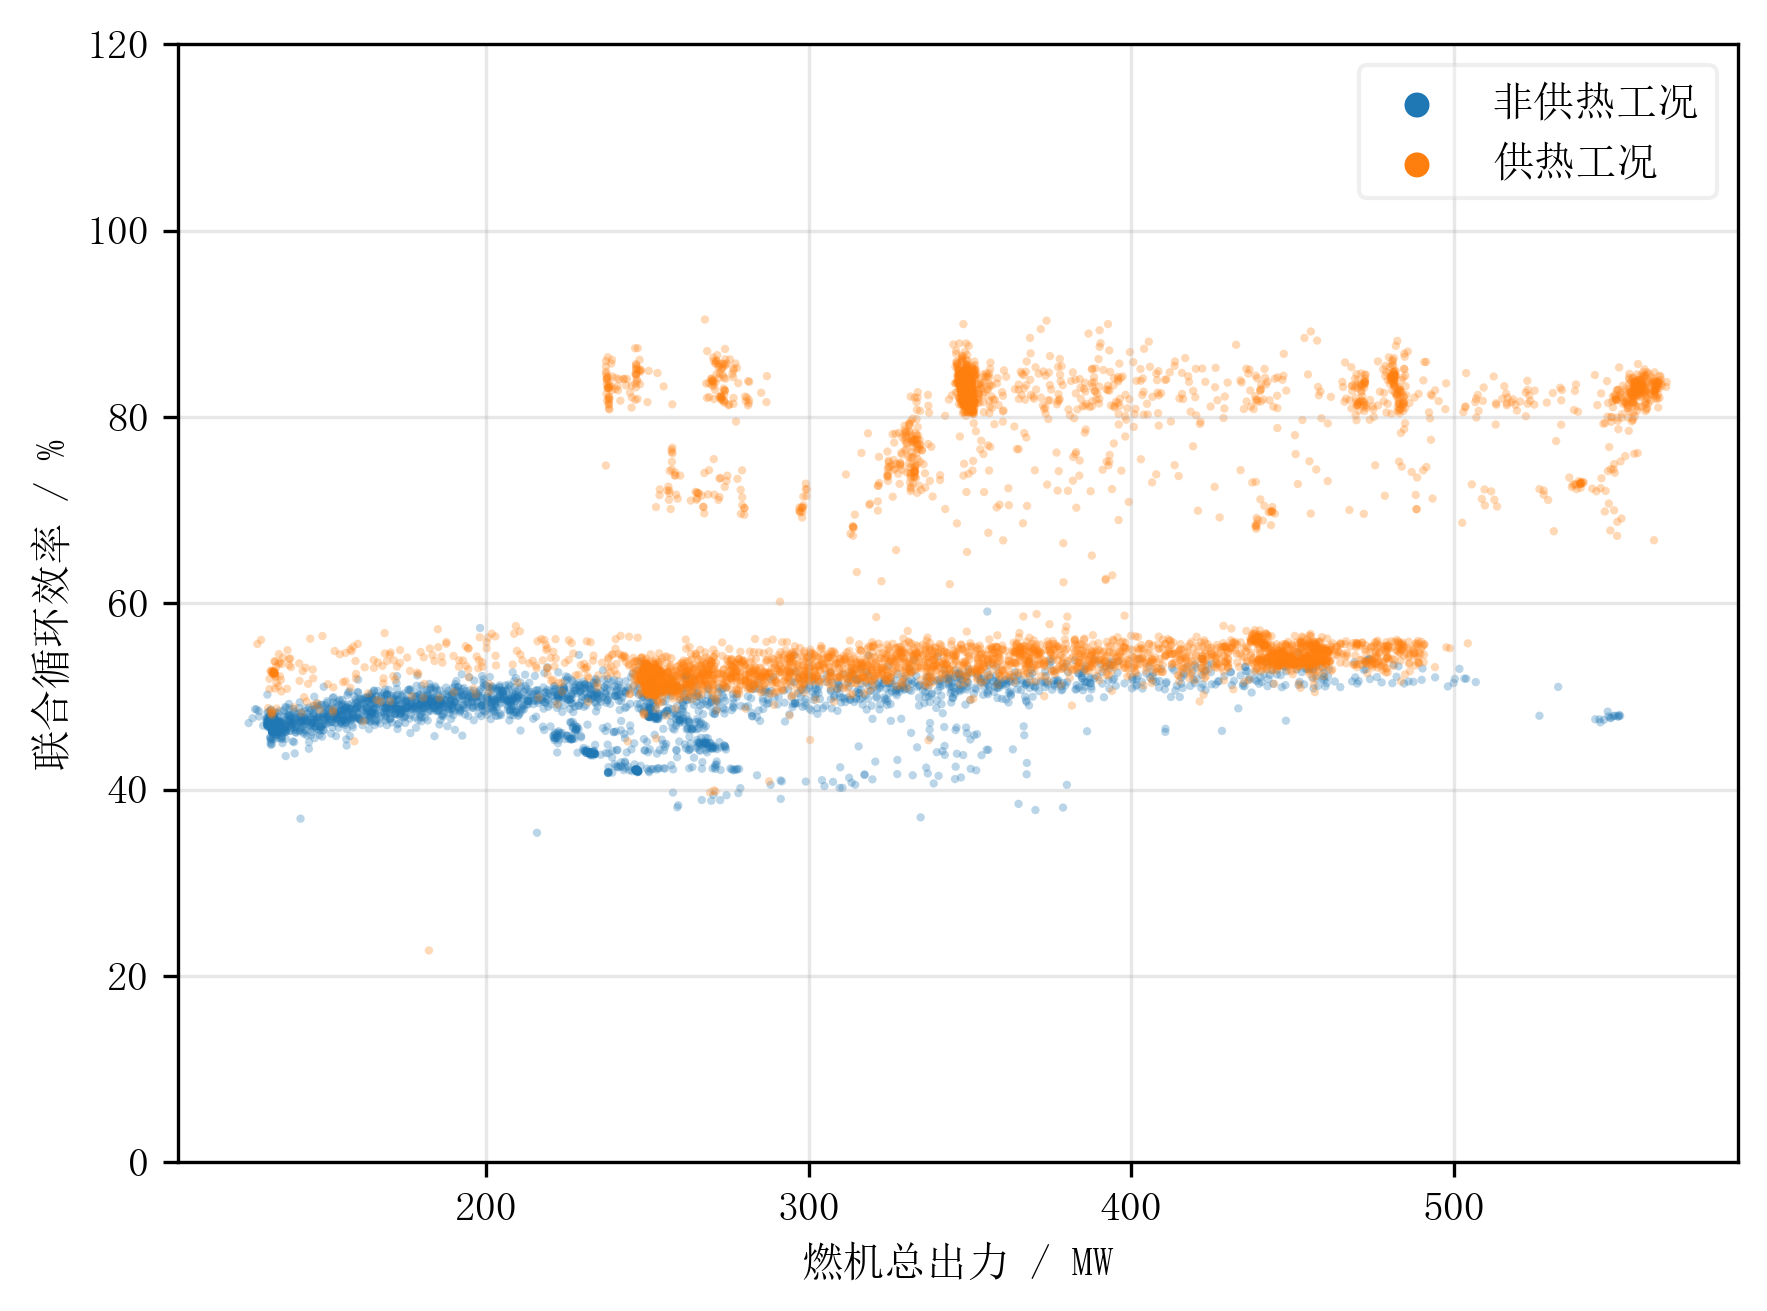
\includegraphics[width=\textwidth]{chapter5/燃机总出力_效率关系.png}
    \caption{Gas turbine output.}
  \end{subfigure}
  \hfill
  \begin{subfigure}{0.48\textwidth}
    \centering
    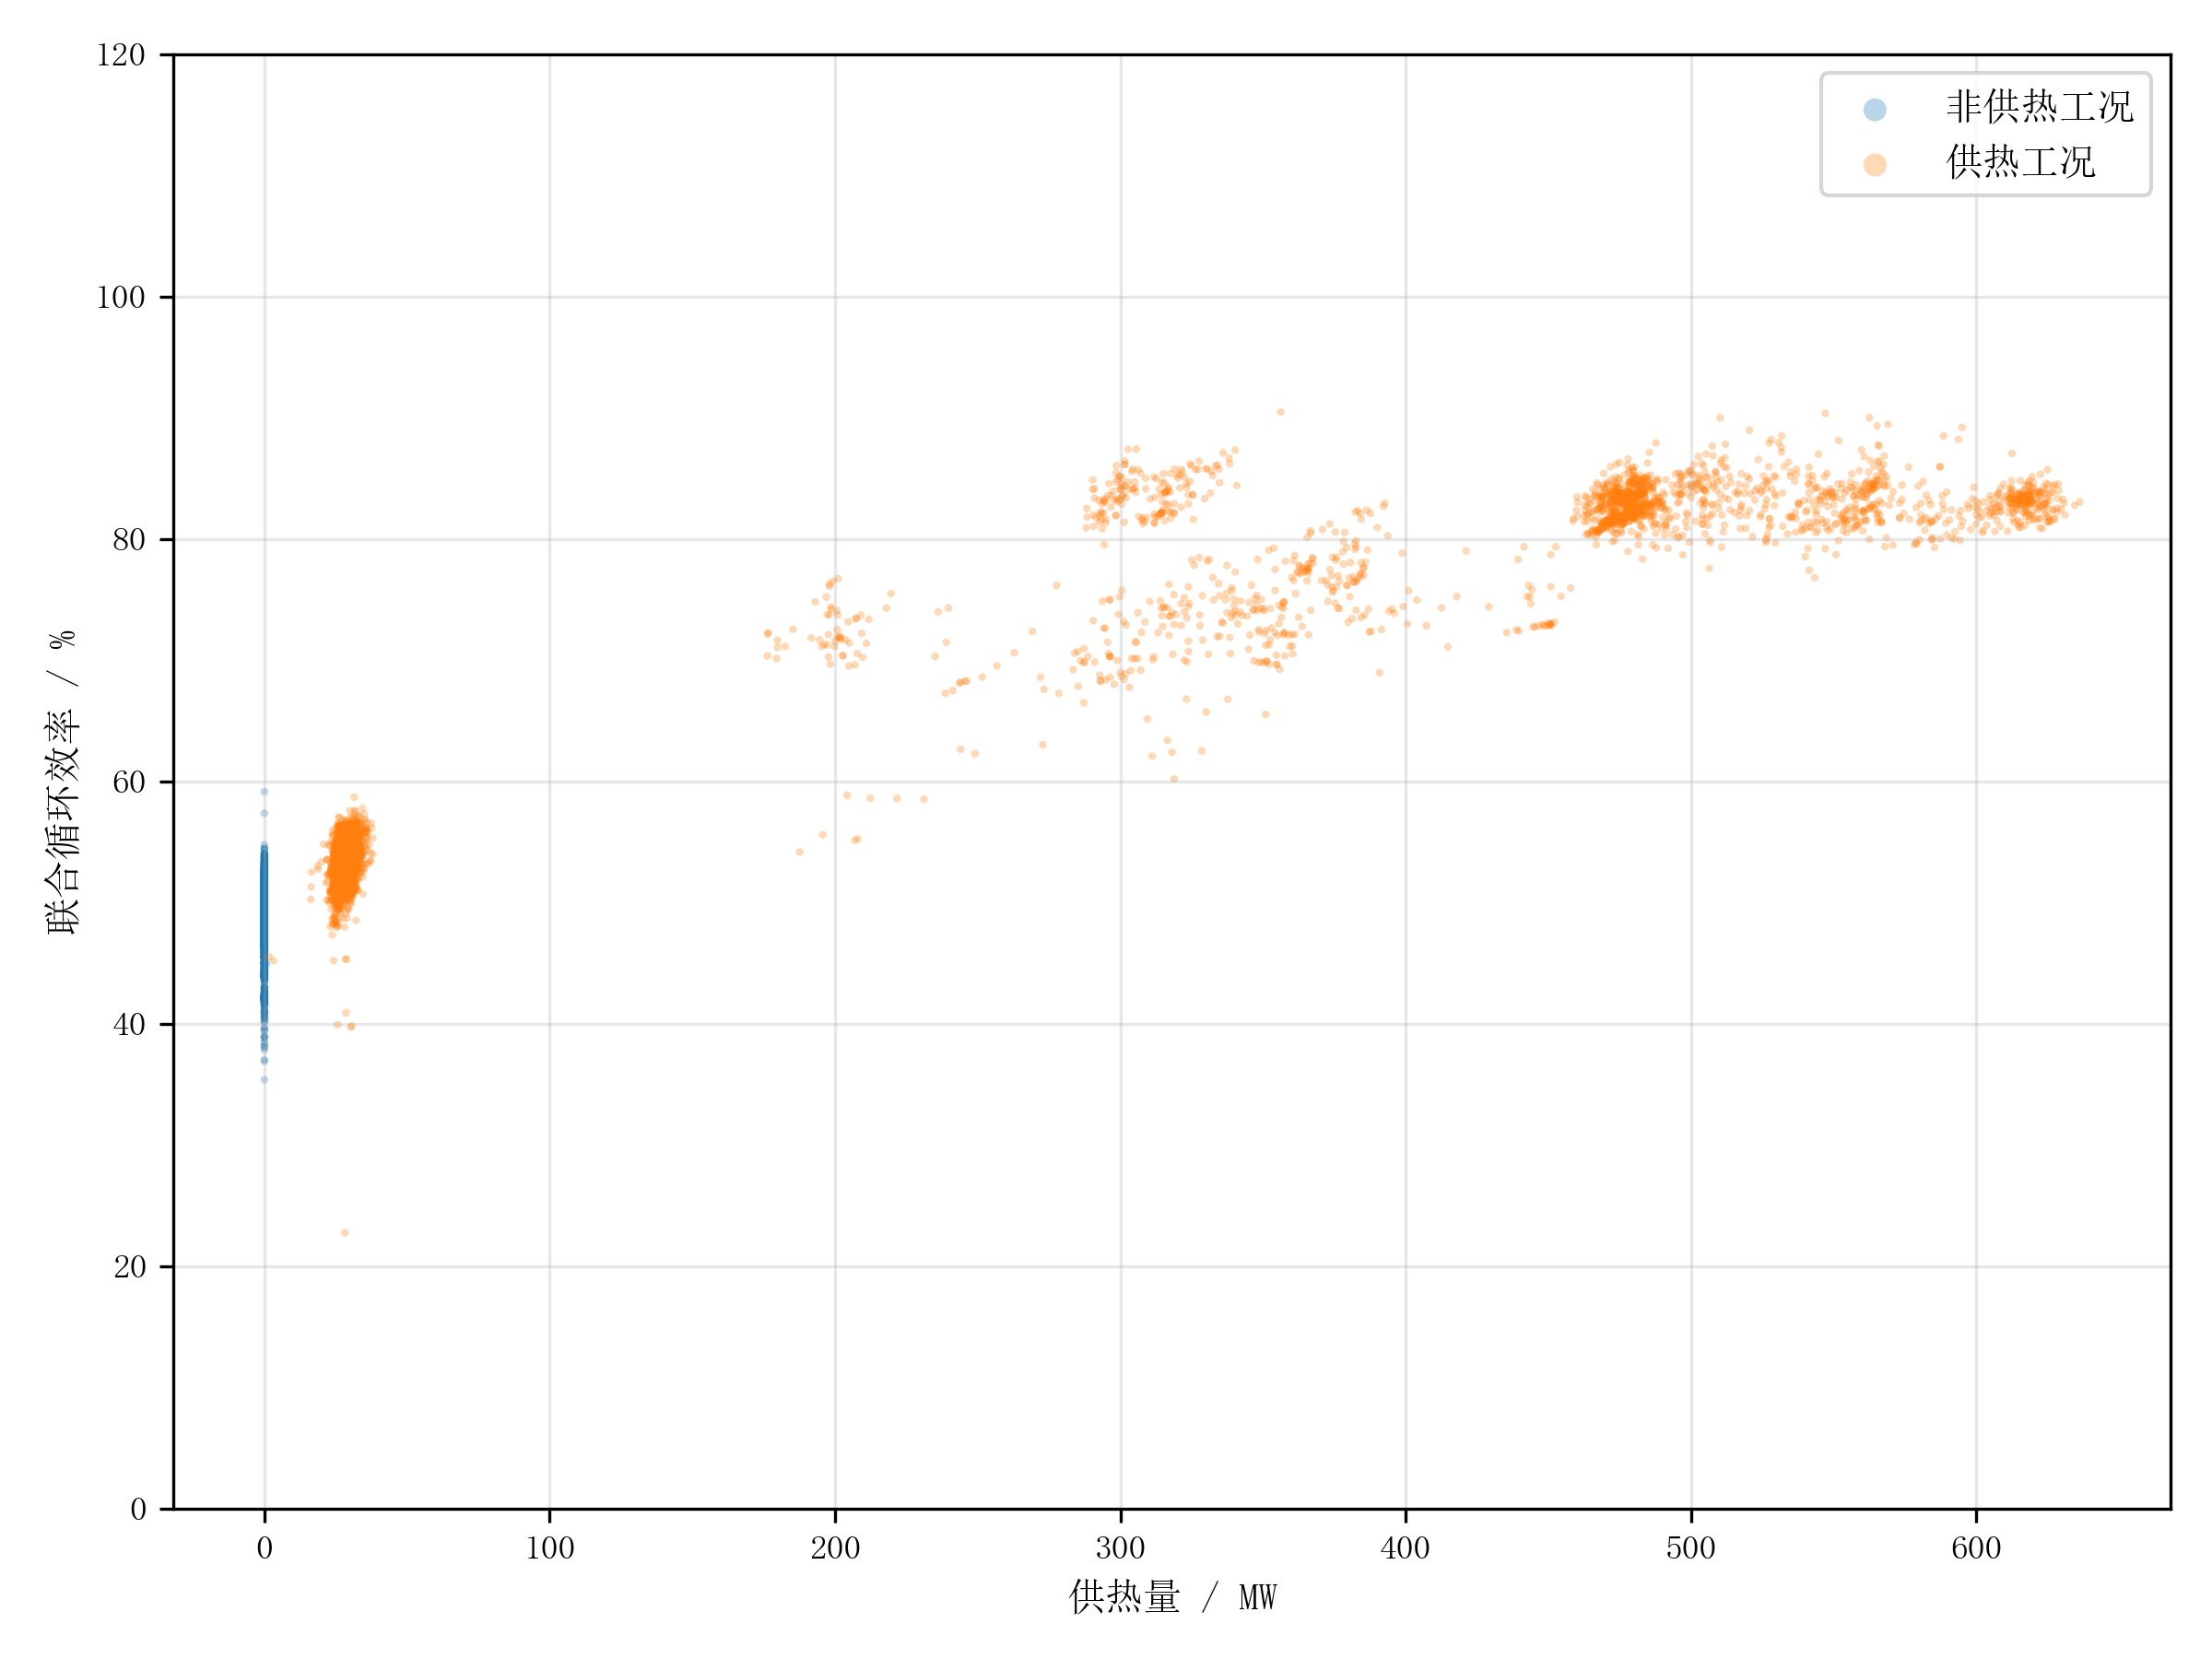
\includegraphics[width=\textwidth]{chapter5/供热量_效率关系.png}
    \caption{Heating load.}
  \end{subfigure}
  \caption{Influence of load level and heating load on efficiency.}
  \label{fig:load-efficiency}
\end{figure}

Ambient variables require careful interpretation. In non-heating operation, ambient temperature is positively correlated with power efficiency and ambient pressure is negatively correlated, which appears inconsistent with a simple gas turbine intake-density mechanism. This reversal is caused by seasonal coupling in the operating data: non-heating samples are concentrated in high-temperature summer periods, during which the unit often operates at high load, and the load effect masks the adverse effect of high inlet temperature. In heating operation, lower ambient temperature increases heat demand, so ambient temperature is strongly negatively correlated with heat-electricity efficiency. Therefore, ambient correlations should be interpreted as combined effects of thermodynamics, seasonal demand and dispatch policy.

\begin{figure}[H]
  \centering
  \begin{subfigure}{0.48\textwidth}
    \centering
    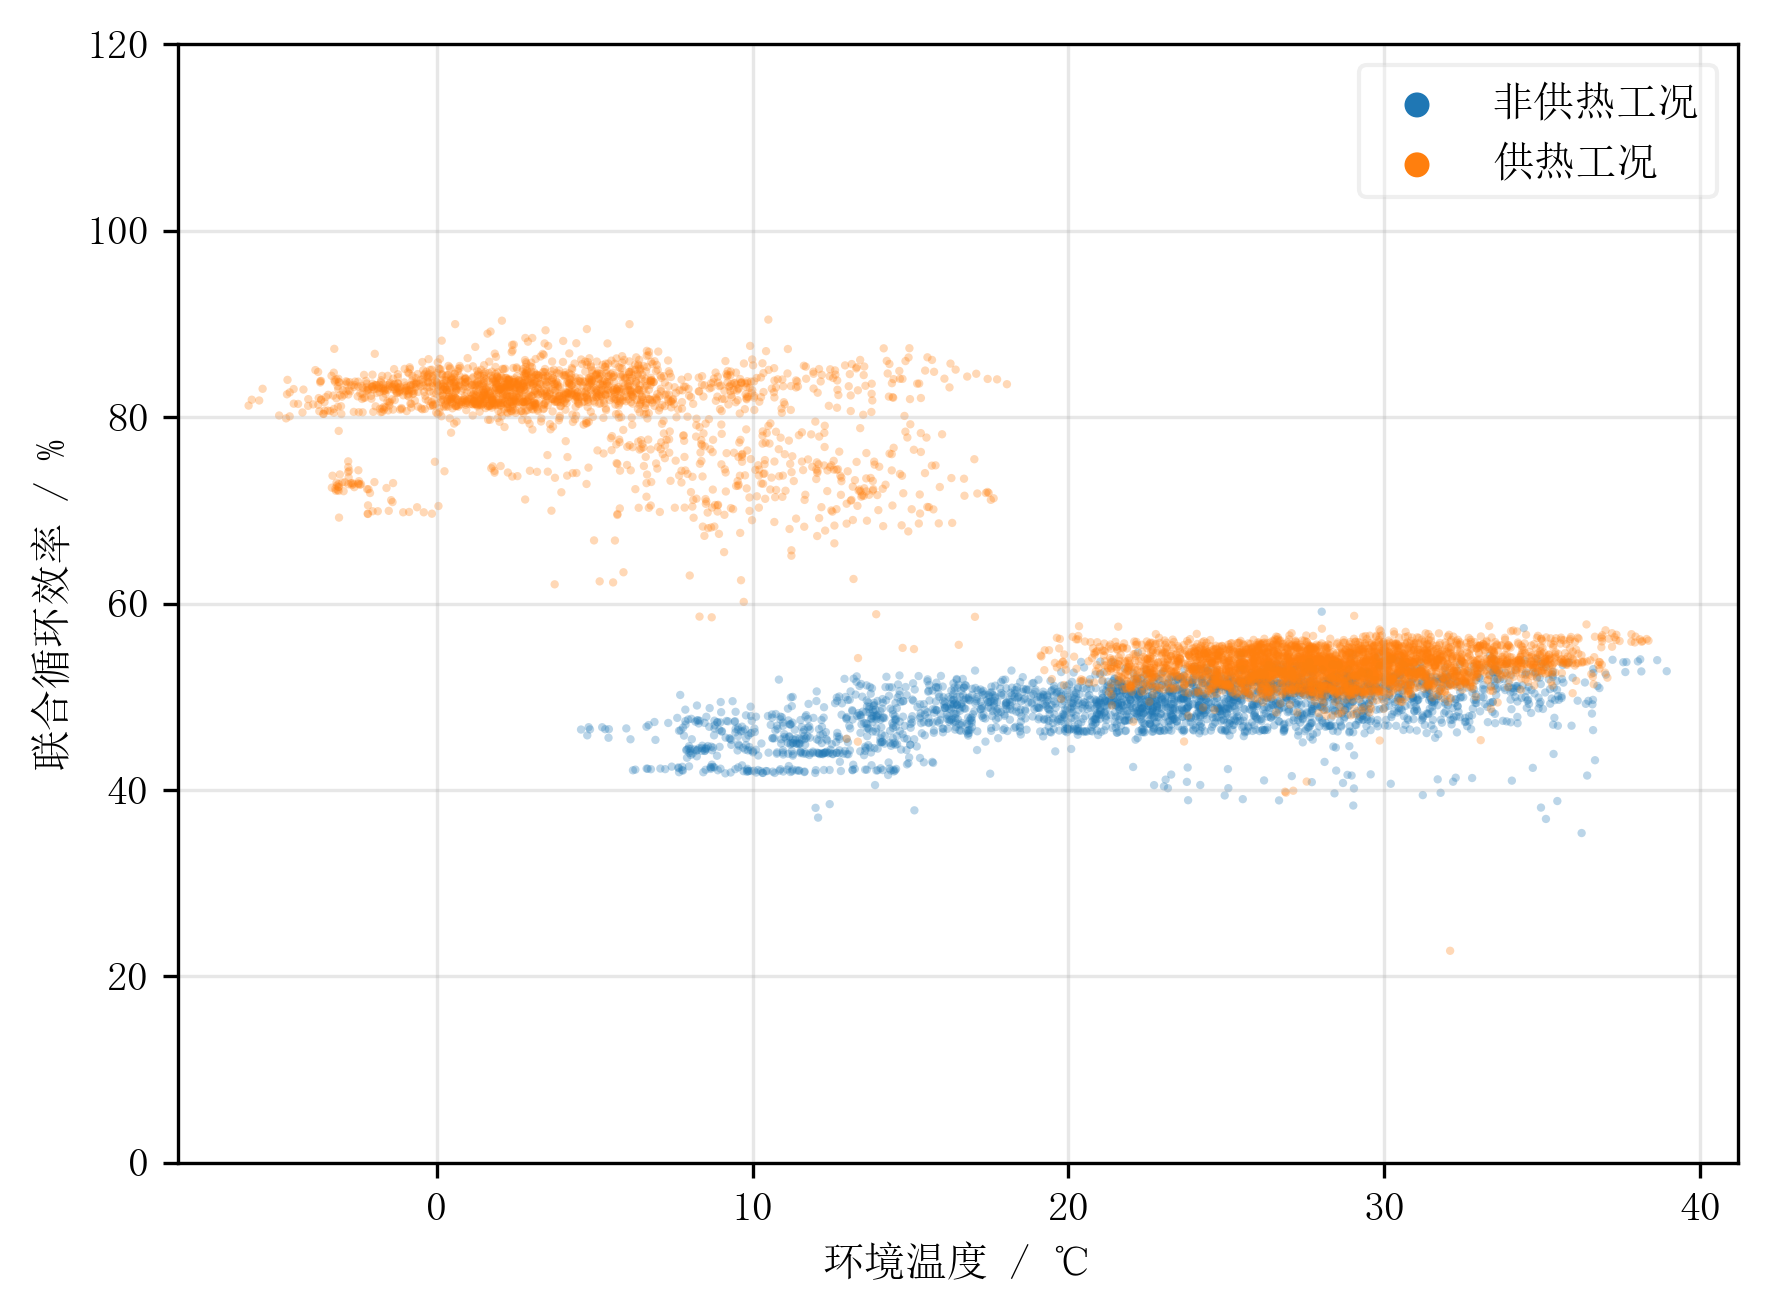
\includegraphics[width=\textwidth]{chapter5/环境温度_效率关系.png}
    \caption{Ambient temperature.}
  \end{subfigure}
  \hfill
  \begin{subfigure}{0.48\textwidth}
    \centering
    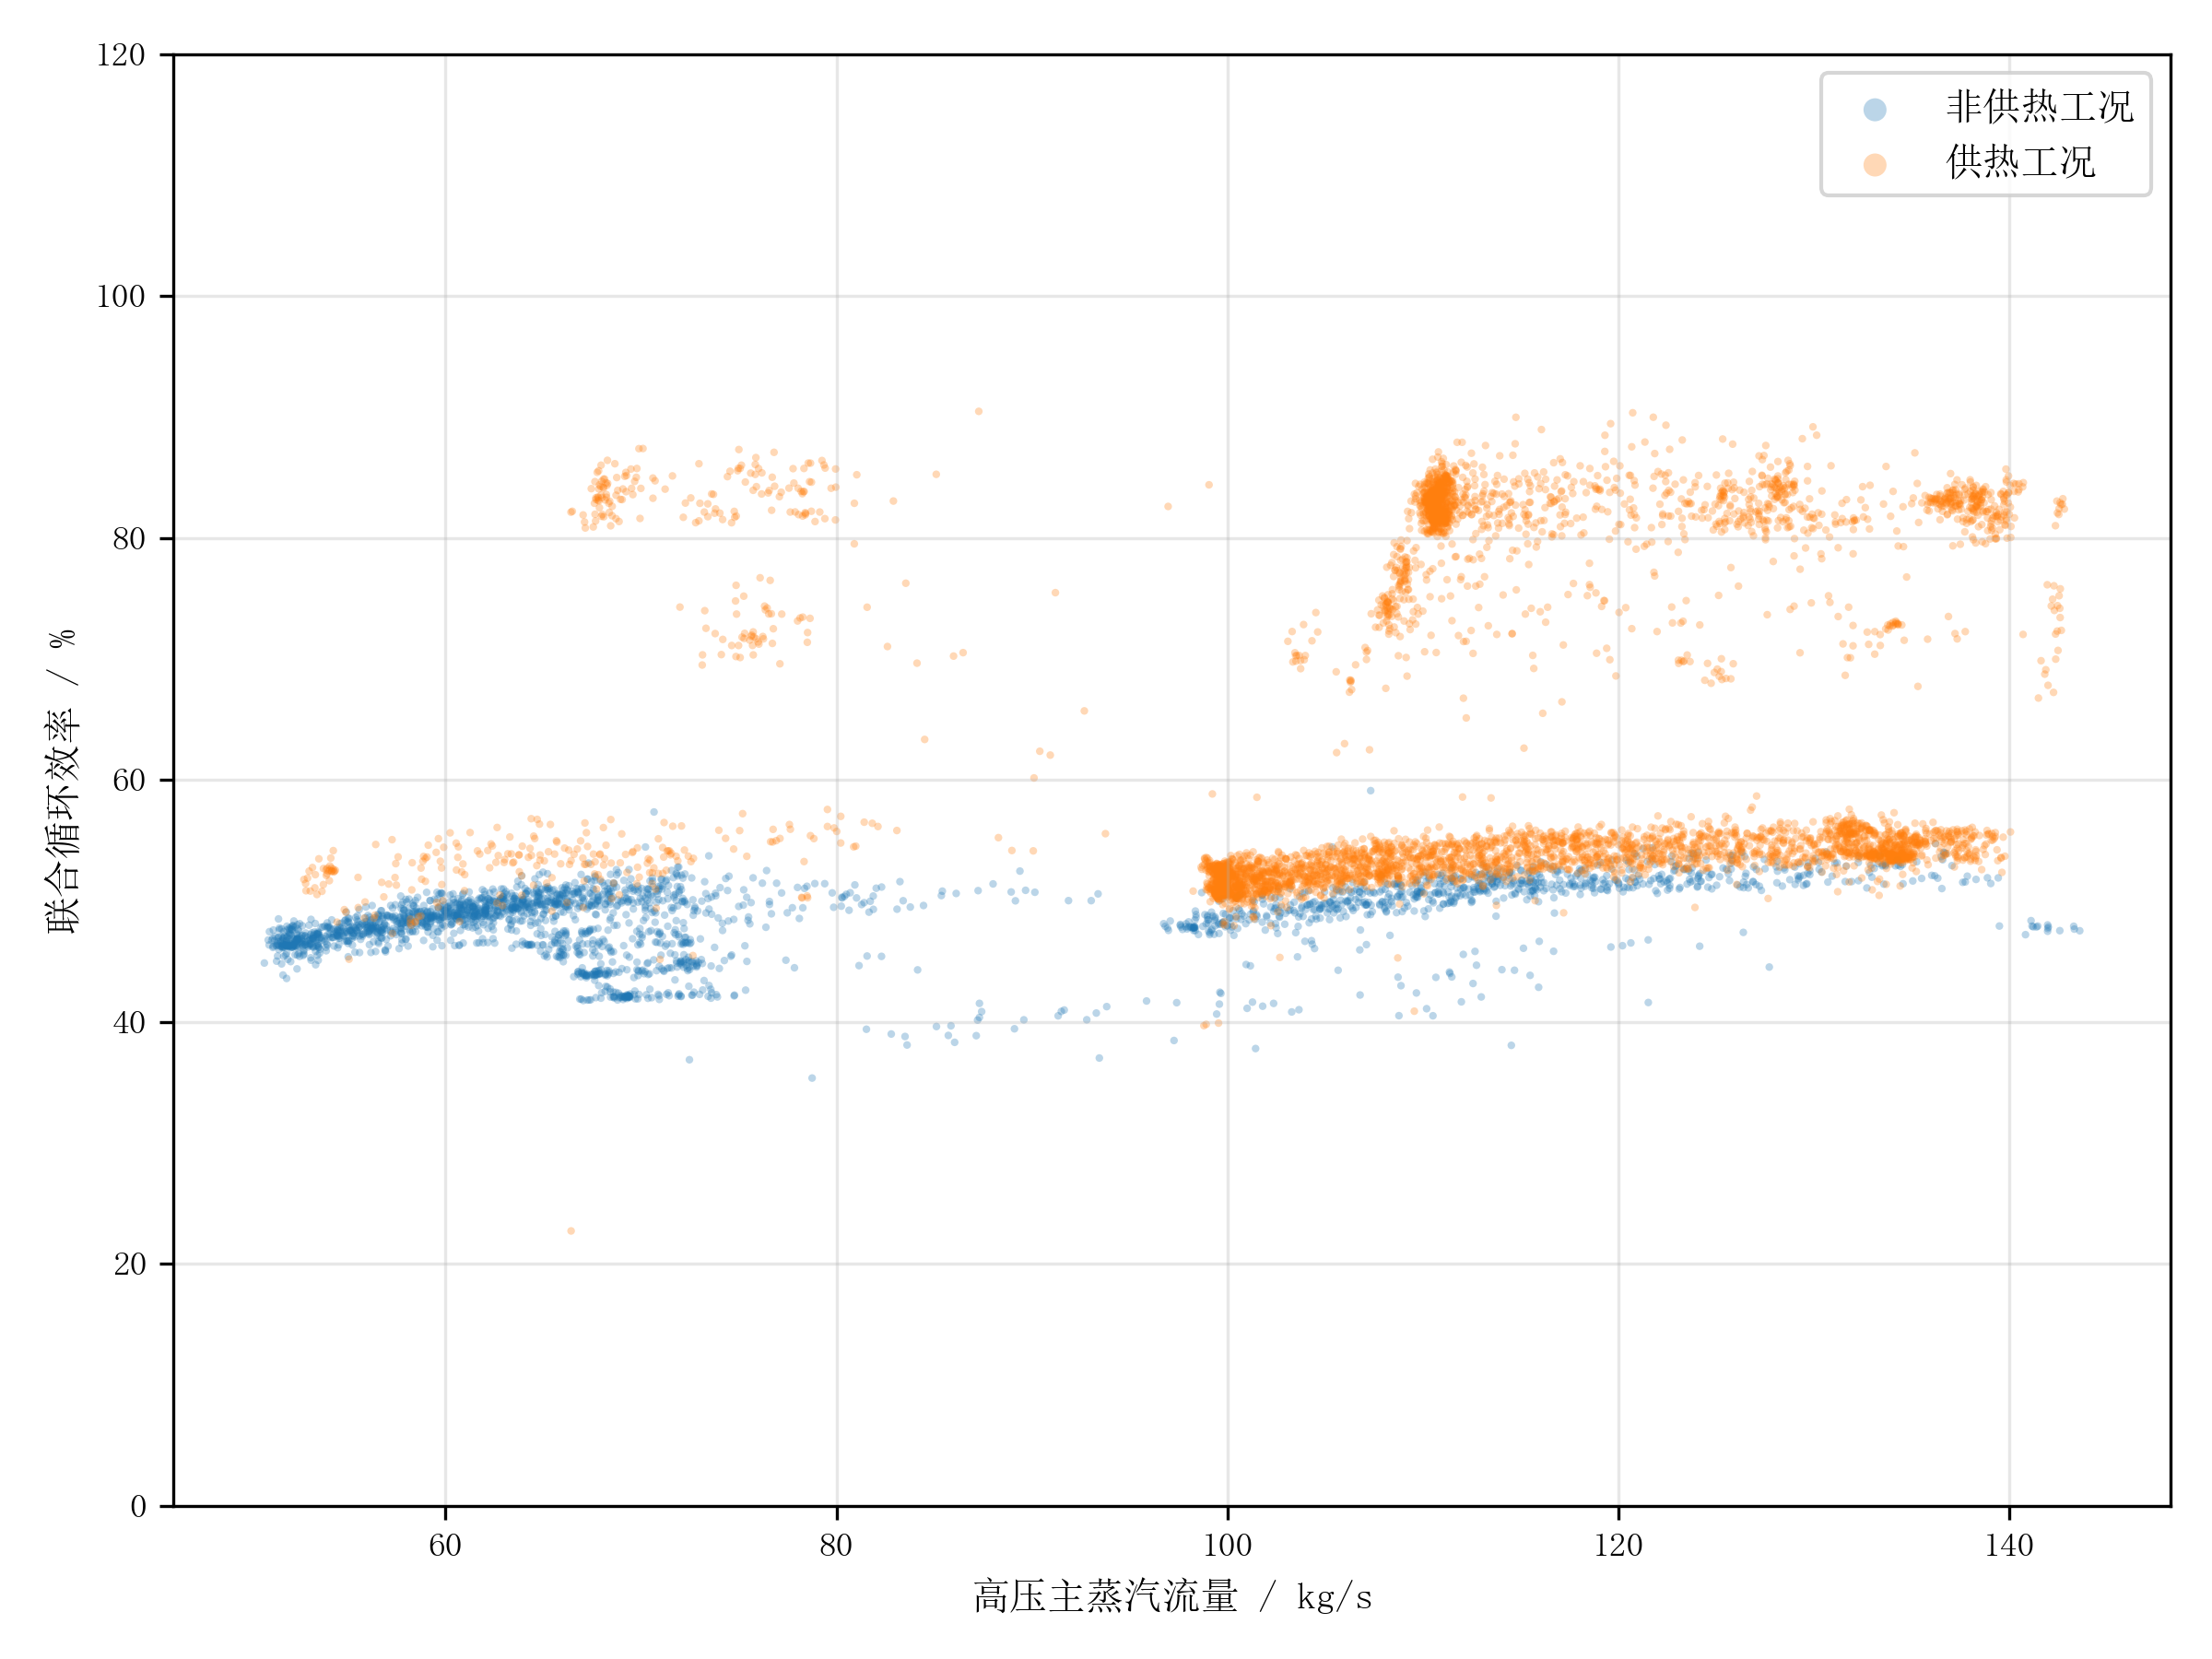
\includegraphics[width=\textwidth]{chapter5/高压主蒸汽流量_效率关系.png}
    \caption{High-pressure main steam flow.}
  \end{subfigure}
  \caption{Representative efficiency-related variables.}
  \label{fig:variables-efficiency}
\end{figure}

\section{Conclusions}

This paper developed a data-driven thermodynamic performance assessment method for a two-on-one gas--steam combined cycle cogeneration unit. The main conclusions are:

\begin{enumerate}
  \item A unified stream model can consistently represent natural gas, humid air, flue gas, water and steam, allowing field measurements to be transformed into thermodynamic states for component-level analysis.
  \item The gas turbine model shows that fuel input is mainly allocated among electric output, compressor consumption and exhaust heat. Electric output accounts for about \(0.28\)--\(0.36\) of fuel input, while exhaust heat remains a major resource for the steam cycle.
  \item HRSG and steam turbine analysis indicates that high-pressure steam heat absorption and HP/IP cylinder output are central to bottoming-cycle power generation. Heating operation redirects low-pressure steam energy from electricity generation to heat supply.
  \item Under non-heating conditions, combined-cycle power efficiency is mainly associated with load level, steam turbine output, main-steam flow, feedwater pressure and heat recovery capability. Under heating conditions, heat-electricity efficiency is dominated by heating load and seasonal ambient conditions.
  \item Pearson correlation analysis is useful for screening influential variables, but its results must be interpreted with component models because load scheduling, seasonality and multicollinearity can reverse apparent correlation directions.
\end{enumerate}

Future work should improve air-flow correction under winter conditions, refine HRSG segment-level heat-transfer modeling, quantify desuperheating and mixing irreversibilities, and extend the framework from performance assessment to operating-condition optimization.

\section*{Acknowledgements}
The author thanks the plant operation data providers and the thesis project supervisors for their support.

\begin{thebibliography}{99}

\bibitem{urban1973gpa}
L. A. Urban, ``Gas path analysis applied to turbine engine condition monitoring,'' \emph{Journal of Aircraft}, vol. 10, no. 7, pp. 400--406, 1973.

\bibitem{stamatis2011gpa}
A. G. Stamatis, ``Evaluation of gas path analysis methods for gas turbine diagnosis,'' \emph{Journal of Mechanical Science and Technology}, vol. 25, no. 2, pp. 469--477, 2011.

\bibitem{tahan2017health}
M. Tahan, E. Tsoutsanis, M. Muhammad, and Z. A. Abdul Karim, ``Performance-based health monitoring, diagnostics and prognostics for condition-based maintenance of gas turbines: A review,'' \emph{Applied Energy}, vol. 198, pp. 122--144, 2017.

\bibitem{hanachi2018survey}
H. Hanachi, C. Mechefske, J. Liu, A. Banerjee, and Y. Chen, ``Performance-based gas turbine health monitoring, diagnostics, and prognostics: A survey,'' \emph{IEEE Transactions on Reliability}, vol. 67, no. 3, pp. 1340--1363, 2018.

\bibitem{kim2004partload}
T. S. Kim, ``Comparative analysis on the part load performance of combined cycle plants considering design performance and power control strategy,'' \emph{Energy}, vol. 29, no. 1, pp. 71--85, 2004.

\bibitem{hyun2018dual}
K. Hyun, T. S. Kim, and J. S. Lee, ``Performance improvement of gas turbine combined cycle power plant by dual cooling of the inlet air and turbine coolant using an absorption chiller,'' \emph{Energy}, vol. 163, pp. 1050--1061, 2018.

\bibitem{yang2019inlet}
Y. Yang, Z. Bai, and G. Zhang, ``Design/off-design performance simulation and discussion for the gas turbine combined cycle with inlet air heating,'' \emph{Energy}, vol. 176, pp. 513--530, 2019.

\bibitem{diakunchak1992deterioration}
I. S. Diakunchak, ``Performance deterioration in industrial gas turbines,'' \emph{Journal of Engineering for Gas Turbines and Power}, vol. 114, no. 2, pp. 161--168, 1992.

\bibitem{kurz2001degradation}
R. Kurz and K. Brun, ``Degradation in gas turbine systems,'' \emph{Journal of Engineering for Gas Turbines and Power}, vol. 123, no. 1, pp. 70--77, 2001.

\bibitem{li2009prognostic}
Y. G. Li and P. Nilkitsaranont, ``Gas turbine performance prognostic for condition-based maintenance,'' \emph{Applied Energy}, vol. 86, no. 10, pp. 2152--2161, 2009.

\bibitem{pinelli2000uncertainties}
M. Pinelli and P. R. Spina, ``Gas turbine field performance determination: Sources of uncertainties,'' \emph{Journal of Engineering for Gas Turbines and Power}, vol. 124, no. 1, pp. 155--160, 2000.

\bibitem{carstens2018uncertainty}
H. Carstens, X. Xia, and S. Yadavalli, ``Measurement uncertainty in energy monitoring: Present state of the art,'' \emph{Renewable and Sustainable Energy Reviews}, vol. 82, pp. 2791--2805, 2018.

\end{thebibliography}

\end{document}
